\documentclass[french, 12pt]{article}
\usepackage[T1]{fontenc}
\usepackage[utf8]{inputenc}
\usepackage{lmodern}
\usepackage[round]{natbib}
\bibliographystyle{unsrtnat}
\usepackage{babel}
\usepackage[colorlinks,citecolor=blue]{hyperref}
\usepackage{mathpazo}
\usepackage{palatino}
\usepackage{booktabs}
\usepackage{graphicx}
\newcommand{\bi}{\begin{itemize}}
	\newcommand{\ei}{\end{itemize}}
\usepackage{xcolor}
\newcommand{\ig}{\includegraphics}
\newcommand{\subt}[1]{{\footnotesize \color{subtitle} {#1}}}
\usepackage{setspace}



%%%%%%%%%%%%%%%%%%%%%%%%%%%%%%%%%%%%%%%%%%%%%%%%%%%%

\title{Revenus de retraite et âge de déclenchement de la rente du RRQ\thanks{\scriptsize Je voudrais remercier Yann Décarie ainsi que Xavier Dufour-Simard pour les calculs réalisés au Centre Interuniversitaire Québécois en Statistiques Sociales (CIQSS) ainsi que le CIQSS et le Réseau des centres de données du Canada qui a permis l'accès aux données fiscales de Statistiques Canada.  
}}
\author{\small Pierre-Carl Michaud\thanks{\scriptsize HEC Montréal, Canada and NBER: pierre-carl.michaud@hec.ca}}
\date{\small \today}



\begin{document}
	
	\maketitle
	
	\begin{abstract}
		\footnotesize 
        Dans cet article, nous analysons le lien entre l'âge de déclenchement de la rente de retraite du RRQ et le revenu disponible (après impôt) une fois à la retraite. Nous exploitons un modèle prédictif de la mortalité estimé sur les données fiscales et en tenant compte des effets du supplément de revenu garanti sur le report de la rente. Nous montrons que l'hétérogénéité d'espérance de vie n'est pas suffisante pour justifier financièrement un âge hatif du début de la rente. Nous montrons que le gain financier du report est grandement affecté par la récupération du SRG qui touche plus de 40\% des cotisants. Malgré cet impact, le rendement alternatif, mesuré par le rendement moyen effectif sur l'épargne demeure faible en comparaison, même sans ajustement pour le risque accrue dans un placement alternatif.  Malgré le fait que plusieurs déclenchent hativement la rente,  nous montrons que ceux-ci atteingnent des les taux de remplacement à la retraite, en terme de revenu après impôt, particulièrement élevés en moyenne au Québec. 
	\end{abstract}

	
	\thispagestyle{empty}
	
	\clearpage
	
	\pagenumbering{arabic}
	\setcounter{page}{1}
	\normalsize 
	
	\onehalfspacing
	
	
	\newpage
	
	
	\section{Introduction}
	
	Il est possible de déclencher le paiement de  sa rente de retraite du RRQ à partir de 60 ans. Il s’agit d’une décision irréversible qui ampute la rente de 36\% comparativement à la valeur de celle-ci si elle est déclenchée à 65 ans. En 2010, près de la moitié des cotisants au Québec déclenchait la rente à 60 ans. Cette proportion a diminué dans les dernières années \citep{michaud2023}. Plusieurs études ont étudié l'optimalité au plan financier de retarder le déclenchement de la rente \citep{milliganschirle2008, michaud2020,macdonald2020,laverdiere2023}.  L'objectif de cet article est d'explorer le lien entre l'âge de déclenchement de la rente et les revenus à la retraite. 
	
	Sous l’angle financier, déclencher sa rente à 60 ans pourrait être avantageux pour ceux ayant un risque de mortalité plus élevé. La pénalité de 36\% pour une déclenchement hatif est calculée par  les actuaires du régime afin que le coût total des prestations que le régime paiera à un cotisant l’ayant débuté à 60 ans plutôt qu’à 65 ans soit le même. Ce calcul peut être fait en utilisant une table de mortalité compilant les statistiques de mortalité de la totalité des cotisants. Si ceux déclenchant la rente à 60 ans n’ont pas le même profil de mortalité, il se peut que le coût pour le régime soit différent. Si ce coût est plus faible, parce que le groupe décède en moyenne plus rapidement, alors le régime épargne de l’argent quand un cotisant déclenche la rente à 60 ans, ce qui veut dire qu’il est avantageux pour le cotisant de retarder. Ce que gagne le cotisant doit être absorbé par le régime.  C'est pourquoi la proposition d'augmenter l'âge minimal pour déclencher la rente, présentée à l'hiver 2023 par le gouvernement du Québec était couteuse pour le régime. 
    
    Le premier objectif de cette note est d'évaluer, à l’aide de données fiscales massives sur les cotisants au Québec, si le profil de mortalité de ceux déclenchant à 60 ans est le même que celui de ceux déclenchant à 65 ans. \citet{milliganschirle2021} ont montré en utilisant des données du RPC que la mortalité étant très différente selon le revenu moyen au cours de la carrière. Nous avons aussi utilisé des profils de mortalité hétérogène basée sur une modélisation par microsimulation dans des études précédentes \citep{glenzer2023,michaud2020}. Or ces profils ne pouvait prendre en compte les améliorations récentes de la mortalité. Nous développons un modèle utilisant les données fiscales récentes, contenant les revenus au dessus du MGA, ainsi que plusieurs autres caractéristiques, incluant une dimension géographique (code postal). Notre premier résultat indique que ceux déclenchant à 60 ans ont une espérance de vie plus faible (un an de moins) que ceux retardant jusqu’à 65 ans. Nous démontrons que le profil de mortalité de ceux déclenchant la rente à 60 ans est très hétérogène. À l'aide d'un modèle prédictif, nous quantifions la distribution du risque de mortalité afin de dégager si certains ont en fait un risque de mortalité suffisament élevé pour justifier de déclencher la rente à 60 ans. Nous montrons que l'espérance de vie moyenne des générations approchant la retraite est si élevée, en ligne avec les projections de l'Institut de la Statistique du Québec,  que même les grandes différences de mortalité entre groupes de la population ne permettent pas de conclure qu'il y a un avantage à prendre la rente à 60 ans
    pour certains. Un résultat similaire a été trouvé pour les États-Unis \citep{shoven_slavov_2014}. Puisque le report de la rente est équivalent à un investissement financier consistant à acheter une rente différée, le rendement implicite du report est très élevé pour ces cotisants. Ceci suggère que le facteur de pénalisation de la rente n'est pas neutre et pourrait être augmenté au cours des prochaines années. 
	
	Le deuxième objectif de cette note est de valider si ceux ayant déclenché la rente à 60 ans ont un taux de remplacement total, incluant toutes les sources de revenu, et après impôts, plus faible que ceux ayant attendu jusqu’à 65 ans? La réponse à cette question est importante puisqu’on cible ce groupe pour potentiellement hausser la couverture contre le risque de longévité et permettre de mieux maintenir leur niveau de vie durant la retraite. Notre deuxième résultat est de montrer que les cotisants déclenchant la rente à 60 ans n'ont pas des taux de remplacement plus faible que ceux la déclenchant à 65 ans. En fait, et de manière assez surprenante, les taux de remplacements sont très élevés au Québec. \footnote{La dernière étude calculant des taux de remplacement similaire utilisait des cotisants ayant atteint l'âge de 65 ans en 2005 \citep{ostrovsky2010}.}  
	
    Le troisième objectif est de vérifier quel serait le gain approximatif pour les cotisants débutant la rente à 60 ans d'attendre jusqu'à 65 ans, sachant que ceux-ci pourrait voir d'autres prestations amputées si la rente du RRQ augmente. Le supplément de revenu garanti exclu la pension de la vieillesse de la récupération mais pas les revenus provenant d'une rente du RRQ. Notre troisième résultat est de montrer que plusieurs cotisants recoivent éventuellement du supplément de revenu garanti à
    la retraite et que l'augmentation de leur prestation du RRQ, si ceux-ci attendait jusqu'à 65 ans, serait accompagnée d'une baisse importante de la prestation provenant du supplément de revenu garanti. Ce résultat n'est pas nouveau. Des simulations ont déjà montré que cet effet potentiel est important \citep{milliganschirle202, michaud2020, laverdiere2023}.  Mais aucune étude n'a quantifié la proportion des gens qui débutent la rente à 60 ans serait sujet à cette récupération s'ils attendaient jusqu'à 65 ans. Nous montrons que cette proportion est importante et varie selon le revenu. Ainsi, cette composante du système de retraite n'aide en rien le report de la rente d'un point de vue financier. Le rendement implicite du report de la rente reste substantiel pour plusieurs mais est beaucoup plus faible pour les cotisants ayant des revenus avant la retraite
    inférieur à la médianne.  Il importe de mentionner que ce rendement effectif doit être comparé au rendement de l'actif qui serait utilisé pour financer la consommation pendant le report. Si cet actif est un RÉER, aussi sujet à la récupération de la SRG, son rendement effectif sera aussi plus faible. Si l'actif est plutôt un CELI, alors le coût d'opportunité est plus élevé puisque celui-ci n'est pas sujet à la récupération de la SRG. Nous avons calculé le rendement effectif que les cotisants de 60 ans ont dans leur CELI à l'aide des données fiscales (pour ceux ayant un CELI). Le rendement réel, après ajustement pour l'inflation, est de 3\% à 4\%.  Pour une grande majorité, et ce même avec la pénalisation du SRG, il apparait profitable de retarder le déclenchement des prestations de RRQ. 
   
 
	\section{Les données}
	
	Pour cette analyse, nous utilisons la DAL, la base de données longitudinales représentant les rapports d'impôts de 20\% de la population canadienne. Nous utilisons des données de 1990 à 2019. Nous nous intéressons aux personnes nées entre 1935 et 1959 pour avoir une expérience de mortalité suffisante. Tous les participants doivent débuter leur rente de RRQ entre 60 et 70 ans. La mortalité débute à 60 ans, et est observée jusqu’à 84 ans (2019-84=1935).  Étant donné notre objectif, une personne est retirée de l’échantillon si elle reçoit une prestation d’invalidité de la RRQ (un programme seulement disponible pour les moins de 65 ans) car ces personnes sont beaucoup plus à risque de décès et débutent presque toutes leur rente de retraite à 65 ans. Nous nous concentrons donc sur les cotisants débutant une rente de retraite. 
	
	Pour les fins de l'analyse, nous contruisons un certain nombre de variables. D'abord, si la personne décède dans la période d'observation, nous avons l'âge de décès. Si cette personne n'est pas décédé à la dernière fois qu'on l'observe dans la DAL, elle est réputée être une observation censurée pour les fins de l'analyse du risque de mortalité. Nous allons comparer la mortalité dans la DAL avec la mortalité projetée par l'ISQ. Nous verrons que la DAL capte bien la mortalité. Nous construisons une variable qui enregistre l'âge où la RRQ est enclenchée en notant l'âge à partir duquel un revenu positif de rente de retraite est enregistré. Notons qu'il est impossible d'exclure les rentes de survivant dans les données fiscales. Il est donc possible que pour certains répondants, nous puissions confondre l'âge de déclenchement de la rente de retraite avec l'âge de déclenchement d'autres prestations du RRQ, tel que la rente du survivant. 
	
	Toutes les autres variables de contrôle sont mesurés à 60 ans ou bien entre 55 et 59 ans. Nous construisons des variables pour le sexe, le statut matrimonial, la cohorte de naissance (génération), le statut d'immigrant (né à l'extérieur du Canada), le code postal regroupé en 125 groupes, un indicateur si le contribuable reçoit des prestations provenant d'un régime de retraite complémentaire (RCR) ou cotise à un tel régime entre 55 et 59 ans. Nous avons un indicateur de l'industrie d'emploi (à deux chiffres) entre 55 et 59 ans. Les secteurs sont seulement disponibles depuis 2000 dans le LAD, donc les personnes sans secteur observé sont regroupées dans un secteur neutre. Notre définition du revenu est le revenu après impôt, que nous transformons en revenu disponible en rajoutant le  retrait net d'un CELI (moins les contributions). Les flux monétaires variables sont en dollars constants de 2015. La variable est discrétisée en vingtiles (20 groupes) sur la base de la distribution dans l'échantillon. Pour notre mesure de la richesse financière, nous considérons les gains/pertes en capitaux auxquels on rajoute les revenus de dividendes, en dollars constants de 2015. Cette variable est divisée en quintiles (malgré ce que son nom suggère), et les personnes sans ces revenus sont attribuées à une sixième catégorie. 
	
	
	
	\section{La mortalité et la rente du RRQ}
	
	Pour obtenir des profils de mortalité, il faut avoir recours à la modélisation puisque la mortalité n'est observée que jusqu'à l'âge de 84 ans et que même si l'échantillon est grand, il ne permet pas de qualifier l'expérience de mortalité selon le profil des cotisants de manière non-paramétrique. Heureusement, la mortalité est bien décrite après l'âge de 60 ans par une loi de Gompertz, ce qui permettra de développer un modèle prédictif. Supposons la probabilité de décès d'un cotisant dans un court lapse de temps $h$ à l'âge $t$, après l'âge de 60 ans, est donnée par 
	
	$$ \lambda_i(t) = \lim_{h \to 0} \Pr(t+h>T_i>t|T>t) = \alpha_{i}\exp\left(\gamma t\right). $$
	
	Ce risque est fonction du temps à travers le paramètre $\gamma$ et d'un facteur spécifique à chaque cotisant, $\alpha_i$.  Sans trop de perte de pouvoir prédictif, nous supposons que la croissance de ce risque avec l'âge est constante entre cotisants mais que le niveau de ce risque est différent selon le cotisant. Par exemple, on supposera que 
	
	$$ \alpha_i = \exp\left(\mathbf{x}_i\beta\right) $$
	
	où $\mathbf{x}_i$ est un vecteur de caractéristiques du cotisant et $\beta$ est un vecteur de coefficients (loadings) influencant le risque individuel $\alpha_i$. La DAL contient un grand nombre d'informations sur les cotisants que nous pouvons utiliser pour prédire le risque $\alpha_i$. Dans le modèle le plus complet que nous utiliserons, il y a plus de 156 variables dans le vecteur $\mathbf{x}$. Nous utilisons l'échantillon des répondants de la DAL qui atteint l'âge de 60 ans à un moment dans la période d'observation entre 1990 et 2019 pour procéder à l'estimation des paramètres par maximum de vraisemblance. 
	
	Le Tableau \ref{tab:hazard} rapporte les résultats d'estimation des paramètres $(\beta,\gamma)$ pour cinq spécifications. Pour les paramètres $\beta$, nous rapportons $\exp(\beta)$, soit le rapport de risque de mortalité. Un facteur inférieur à un indique que le risque est plus faible et vice versa pour un risque plus élevé. Sans surprise le risque de décès est plus élevé chez les hommes, chez ceux vivant seul et pour les générations plus âgés. Dans une spécification qui contrôle pour le revenu, cet effet de génération est éliminé. On trouve également que les contribuables nés à l'extérieur du Canada ont une mortalité plus faible. Le risque de mortalité augmente avec l'âge comme on pourrait s'y attendre (le paramètre $\gamma$).  
	
	
	\begin{table}[!htbp]
		\centering
		\small
		\begin{tabular}{lccccc}
			\toprule
						   & (1) 		& (2) 		& (3) 		& (4) 		& (5) 		\\
		\midrule
		Homme  			   & 1.747 		& 1.741 	& 1.765 	& 1.825 	& 2.005 	\\
		(ref. Femme)	   & (0.021)	& (0.021) 	& (0.020) 	& (0.020) 	& (0.021)	\\
		En union		   & 0.756		& 0.751		& 0.757		& 0.770		& 0.812 	\\
		(ref. celibataire) & (0.001)	& (0.010)	& (0.010)	& (0.010)	& (0.011) 	\\
		Générations  &			& 			& 			& 			& 			\\
		(ref. 1945-1950) &&&&&\\
		1935-1939		   & 1.036		& 1.036		& 0.992		& 0.877		& 0.885	 \\
						   & (0.018)	& (0.019)	& (0.018)	& (0.016)	& (0.016) \\
		1940-1944		   & 1.021		& 1.020		& 0.998		& 0.958		& 0.937	 \\
						   & (0.017)	& (0.017)	& (0.017)	& (0.016)	& (0.016) \\
		1950-1954		   & 0.939		& 0.937		& 0.959		& 0.958		& 0.948	 \\
						   & (0.021)	& (0.021)	& (0.022)	& (0.021)	& (0.021) \\
						 
		1955-1959		   & 0.930		& 0.924		& 0.952		& 0.943		& 0.919	 \\
						   & (0.039)	& (0.039)	& (0.040)	& (0.039)	& (0.038) \\
	
						
		Immigrant		   & 0.640		& 0.660		& 0.648		& 0.647		& 0.632	 \\
						   & (0.014)	& (0.015)	& (0.015)	& (0.016)	& (0.015) \\
					
						
		Contributions RCR  & 			& 		& 0.815		& 0.923		& 1.019	 \\
						   & 			& 		& (0.010)	& (0.013)	& (0.016) \\
						   
						  
		Revenus RCR		   & 			& 			& 1.072		& 1.036		& 1.084	 \\
						   & 			& 			& (0.015)	& (0.015)	& (0.016) \\
						   
						   
		\midrule
		Effets fixes 	   &&&&&\\
		Codes postaux	   & 			& $\times$	& $\times$  & $\times$	& $\times$ \\
		Frais médicaux	   & 			& 			& $\times$  & $\times$	& $\times$ \\
		Industrie	  	   & 			& 			& 		    & $\times$	& $\times$ \\
		Vintiles revenu	   & 	& 	&   & 	& $\times$ \\
		Quntiles capitaux &			& 			& 			& 			& $\times$ \\
		\midrule 
		$\gamma$ 		   & 0.132		& 0.131 	& 0.132 	& 0.132		& 0.131  \\  
						   & (0.001)	& (0.001)	& (0.001)	& (0.001)	& (0.001) \\
		\midrule 
		AIC 			   & 203615		& 203440	& 202911	& 201854	& 201110 \\
		N 				   & 330945 	& 330945 	& 330945 	& 330945 	& 330945 \\
		\bottomrule
		\end{tabular}
		\caption{\textbf{Déterminants du risque de mortalité ches les Québécois après l'âge de 60 ans}: Le tableau rapporte les coefficients $\beta$ en forme de risque relatif, $\exp(\beta)$, ainsi que les écart-types. Chaque spécification utilise un nombre différents de caractéristiques $\mathbf{x}$. Les coefficients provenant des effets fixes ne sont pas présentés, car trop nombreux. Le paramètre $\gamma$ measure la pente du risque de mortalité avec l'âge. Finalement AIC est le critère d'information d'Akaike, une mesure du pouvoir prédictif du modèle qui pénalise un nombre trop nombreux de paramètres à estimer.}
		\label{tab:hazard}
	\end{table}
	
	À la Figure \ref{fig:gradient}, nous mettons en evidence le gradient de la mortalité avec le revenu en montrant les risques relatifs par niveau de revenu avant 60 ans. Ceux dans le dernier vingtile de revenus (top 5\%), ont un risque de mortalité 30\% plus faible que ceux à la médiane. 
	
	\begin{figure}[!htbp]
		\centering
		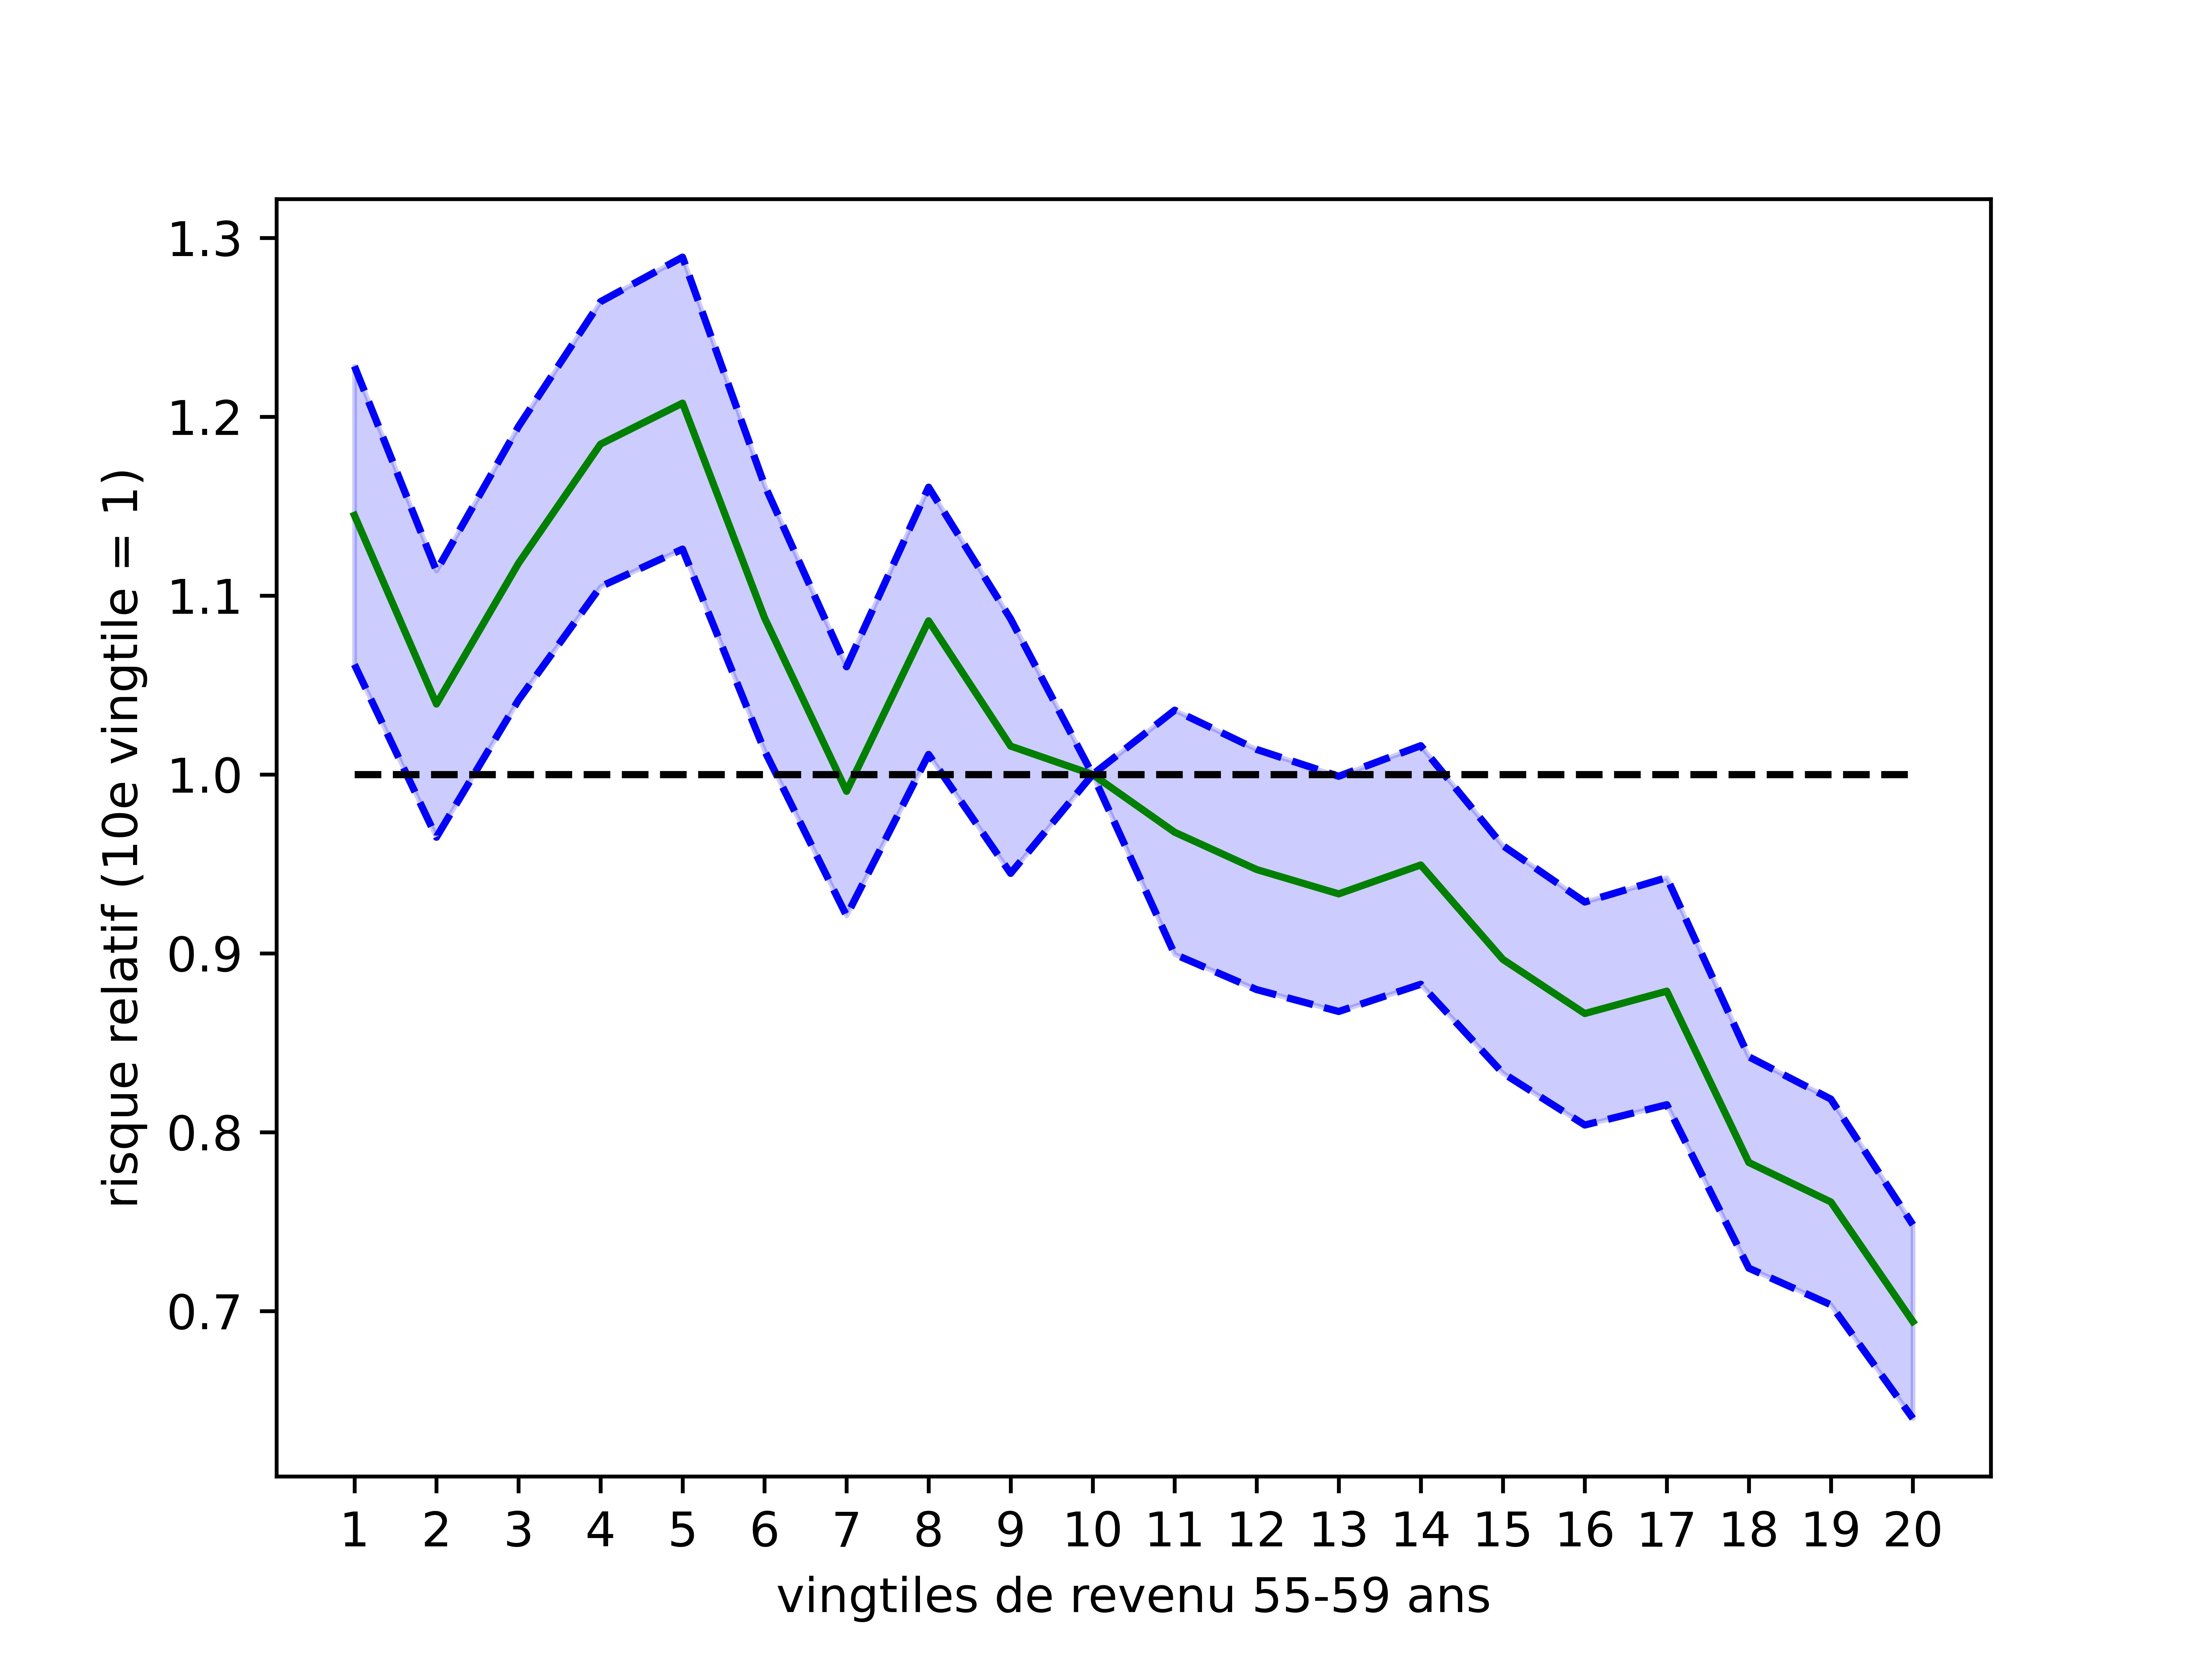
\includegraphics[scale=0.75]{../figures/gradient.png}
		\caption{\textbf{Risque relatif de décès selon le revenu}: Le risque relatif est obtenu à partir des paramètres $\beta$ obtenu dans la spécification (5) du Tableau \ref{tab:hazard}. Ces risques relatifs sont exprimés par rapport au 10e vingtile (incluant la médiane) de la distribution des revenus moyens entre l'âge de 55 et 59 ans au Québec. Les intervales de confiance sont présentés.}
		\label{fig:gradient}
	\end{figure}
	
	Avec ces estimations, on peut calculer une prédiction de $\alpha_i$ pour chacun des cotisants et donc une distribution de $\alpha_i$. Ceci permet d'obtenir une fonction de répartition $F_N(\alpha_i)$ dans l'échantillon. Le $p$ percentile de la distribution est $\alpha_p = F_N^{-1}(p)$ où $F_N^-1(\cdot)$ est la fonction de répartition inverse. Les prédictions sont effectuées sur une portion plus récente de l’échantillon, soit les personnes nées entre 1945 et 1954 (qui ont 60 ans de 2005 à 2014). Pour caractériser les différences de mortalité, nous allons passé à l'espérance de vie à 60 ans. Pour ce faire, nous avons besoin de calculer le taux de survie à chaque âge, à partir de 60 ans. Soit $t = 0$ à 60 ans. Nous avons que le taux de survie est donné par 
	
	$$ s_i(t) = \exp\left(-\alpha_{i}\int_{0}^t \exp\left(\gamma z\right)dz\right) = \exp\left(-\frac{\alpha_{i}}{\gamma}\left(\exp\left(\gamma t\right)-1\right)\right) $$
	
	L'espérance de vie à 60 ans est donnée par
	
	$$ e_{i}(60) = \int_0^{\infty} s_i(z)dz $$
	
	La Figure \ref{fig:ex} montre la fonction de répartition de ces espérances de vie restante. Ainsi plus de 20\% des cotisants âgées de 60 ans ont une espérance de vie restante de plus de 30 ans. Étant donné l'âge de départ de 60 ans, ceci veut dire que plus de 20\% de cette population a un âge espéré de décès de plus de 90 ans. Le moyenne se situe à 27.5 ans, donc un âge de décès moyen de 87.5 ans. 
	
	\begin{figure}[!htbp]
		\centering 
		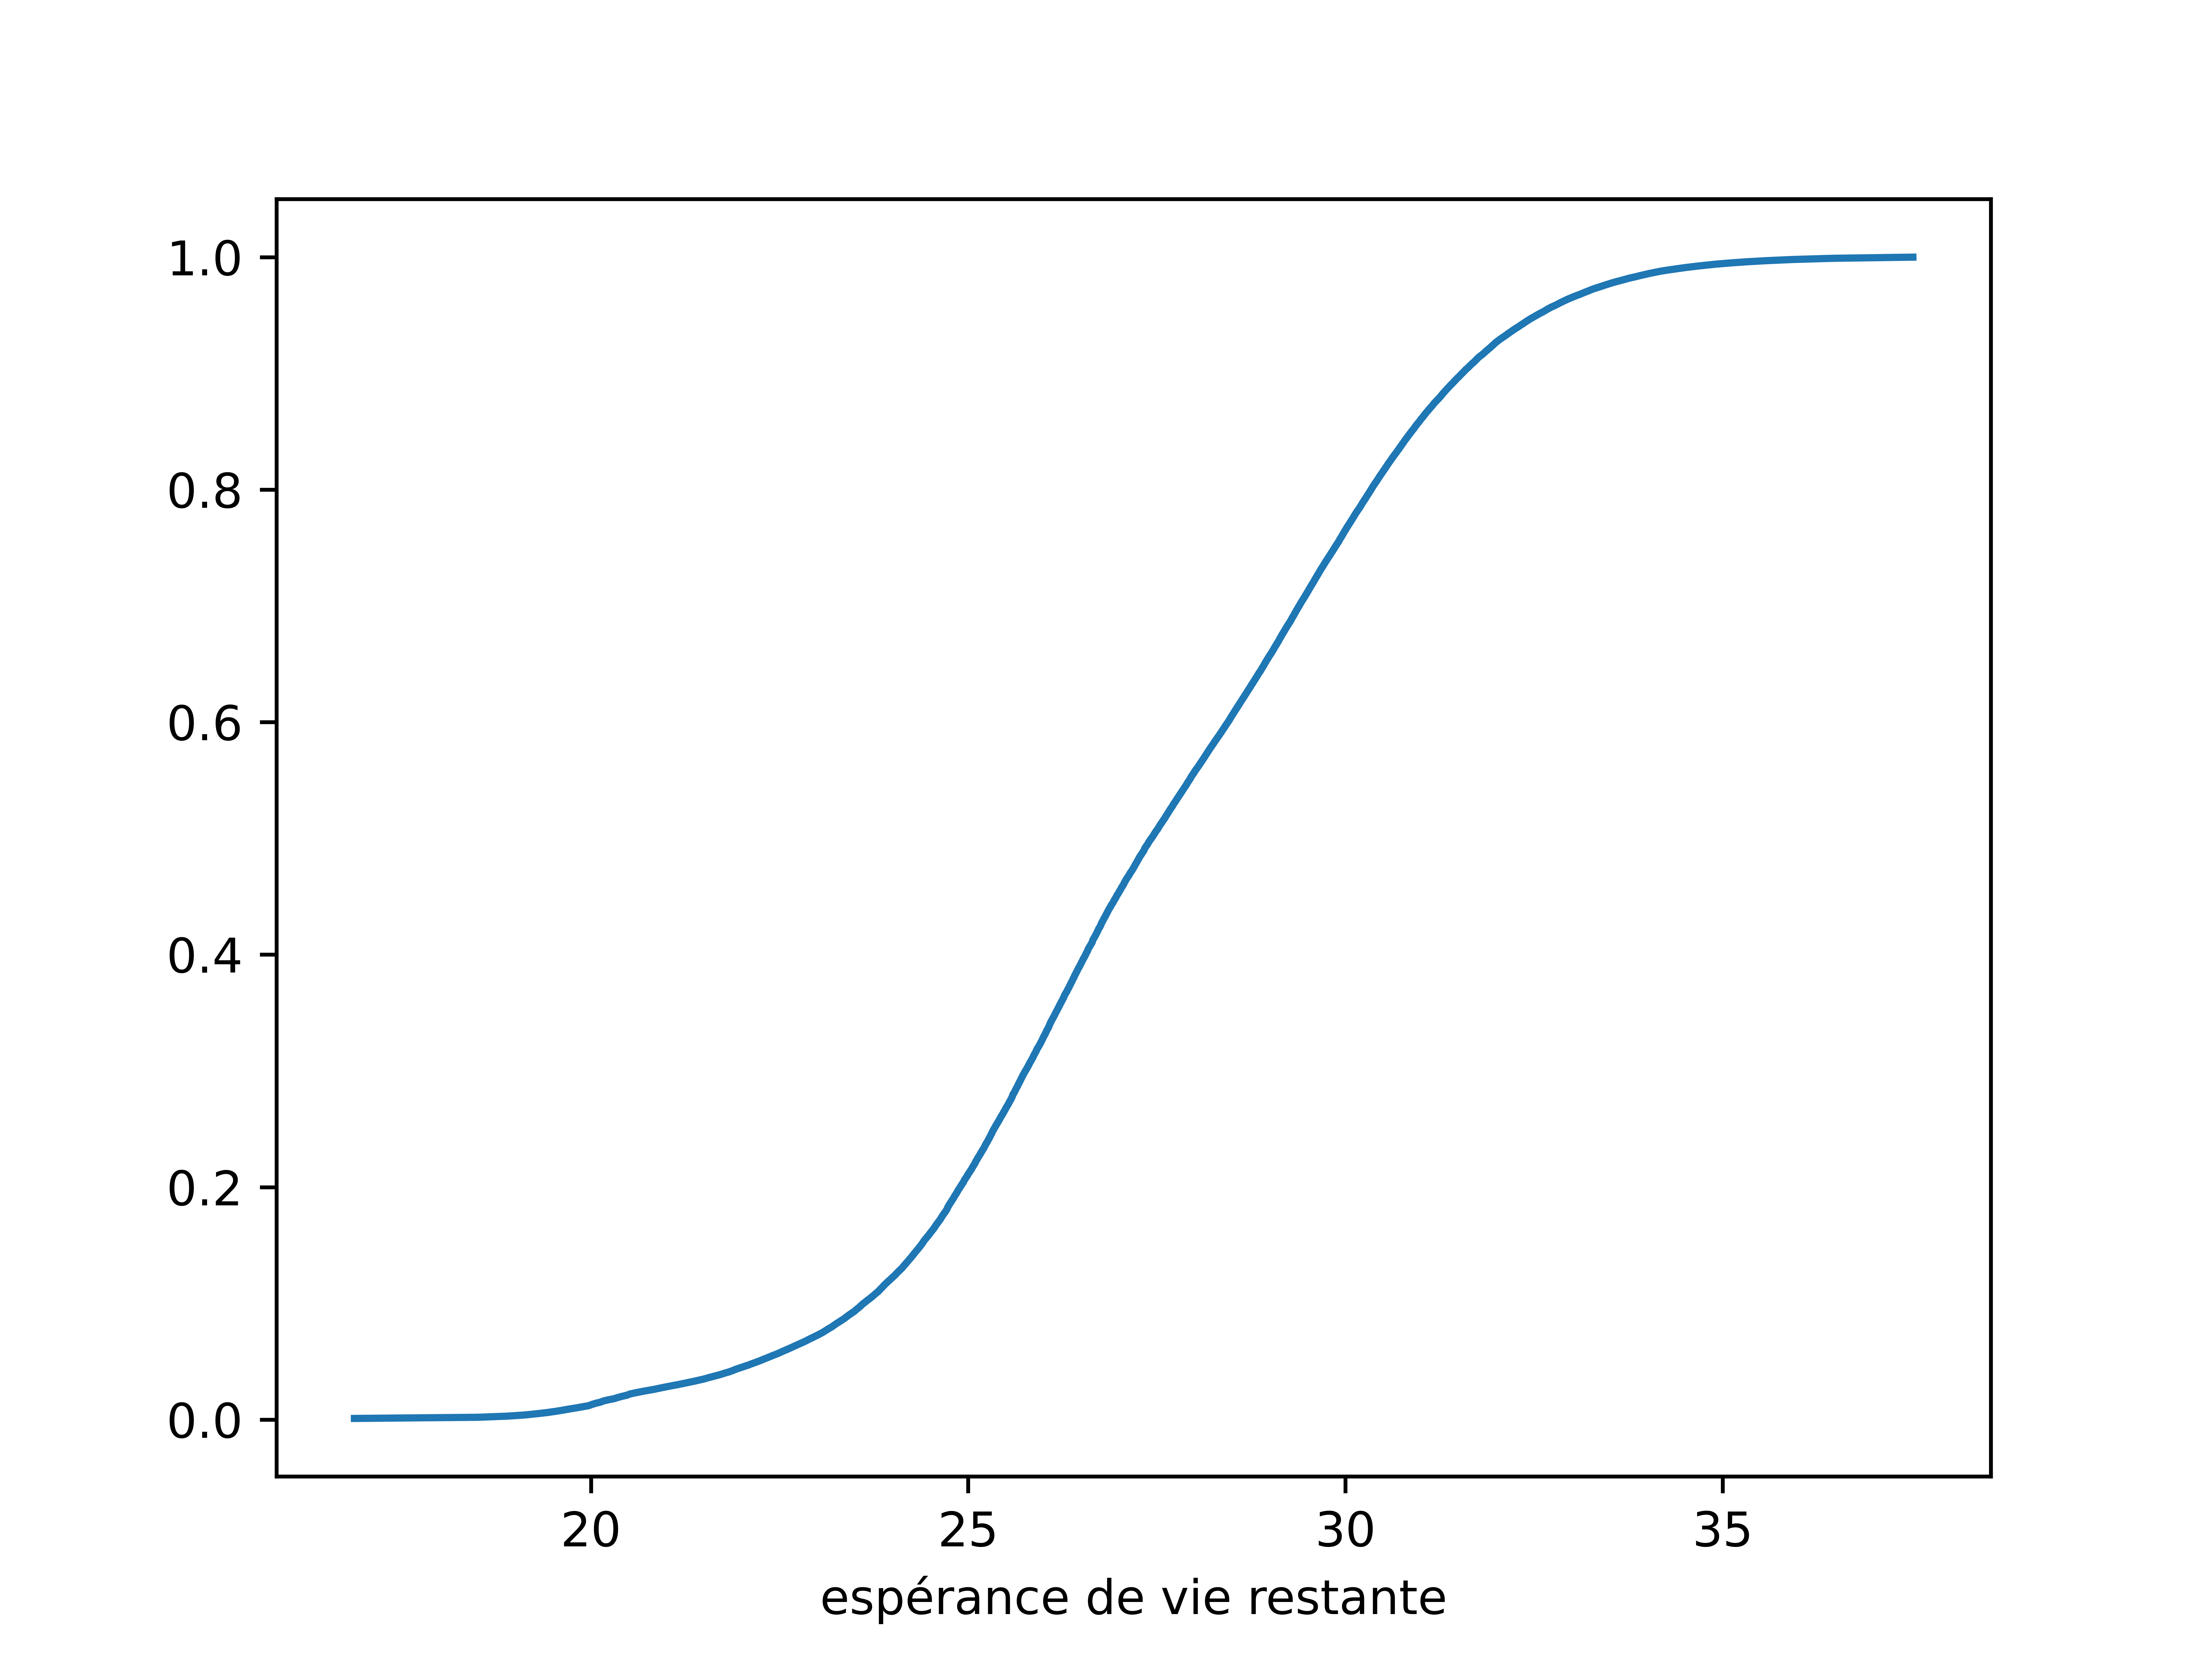
\includegraphics[scale=0.75]{../figures/ex.png}
		\caption{\textbf{Distribution des espérances de vie restante - LAD}}
		\label{fig:ex}
	\end{figure}
	
	Il est important de valider que ces espérances de vie, en particulier la moyenne, sont cohérentes avec les projections de la mortalité produire par les démographes. Pour ce faire, nous utilisons les projections produites par l'Institut de la Statistique du Québec par génération. Nous utilisons les risques relatifs calculés sur la DAL, $\alpha_i$ et nous appliquons ensuite les quotients de mortalité de l'ISQ pour les mêmes générations. Le Tableau \ref{tab:compare} montre que les espérances de vie sont très similaires. Donc, notre modèle estimé sur le LAD est cohérent avec les projections de l'ISQ. 
	
	\begin{table}[!htbp]
		\centering
		\begin{tabular}{lrrrr}
			\toprule 
				& Moyenne & 10 perc. & Médianne & 90 perc \\
			\midrule
			ISQ & 27.7 & 23.1 & 27.4 & 32.5 \\
			LAD & 27.5 & 23.6 & 27.6 & 31.5 \\
			\bottomrule
		\end{tabular}
		\caption{\textbf{Comparaisons espérances de vie restante ISQ - LAD}}
		\label{tab:compare}
	\end{table}
	
	
	Notre premier objectif est de regarder si le risque moyen de mortalité est différent selon l'âge de déclenchement de la RRQ. Pour ce faire, nous pouvons regarder la moyenne des espérances de vie restante par âge de déclenchement. La Figure suivante montre la moyenne et des percentiles pour chacun des âges de déclenchement de 60 à 70 ans. On observe que les cotisants déclenchant la rente à 60 ans ont une espérance de vie légèrement plus faible que ceux déclenchant à 65 ans. Mais la différence est de moins d'une année. Par rapport à la variation de ces espérances de vie observée (en zone ombragée dans la Figure), ces différences sont plutôt faibles. 
	
	\begin{figure}[!htbp]
	\centering 
	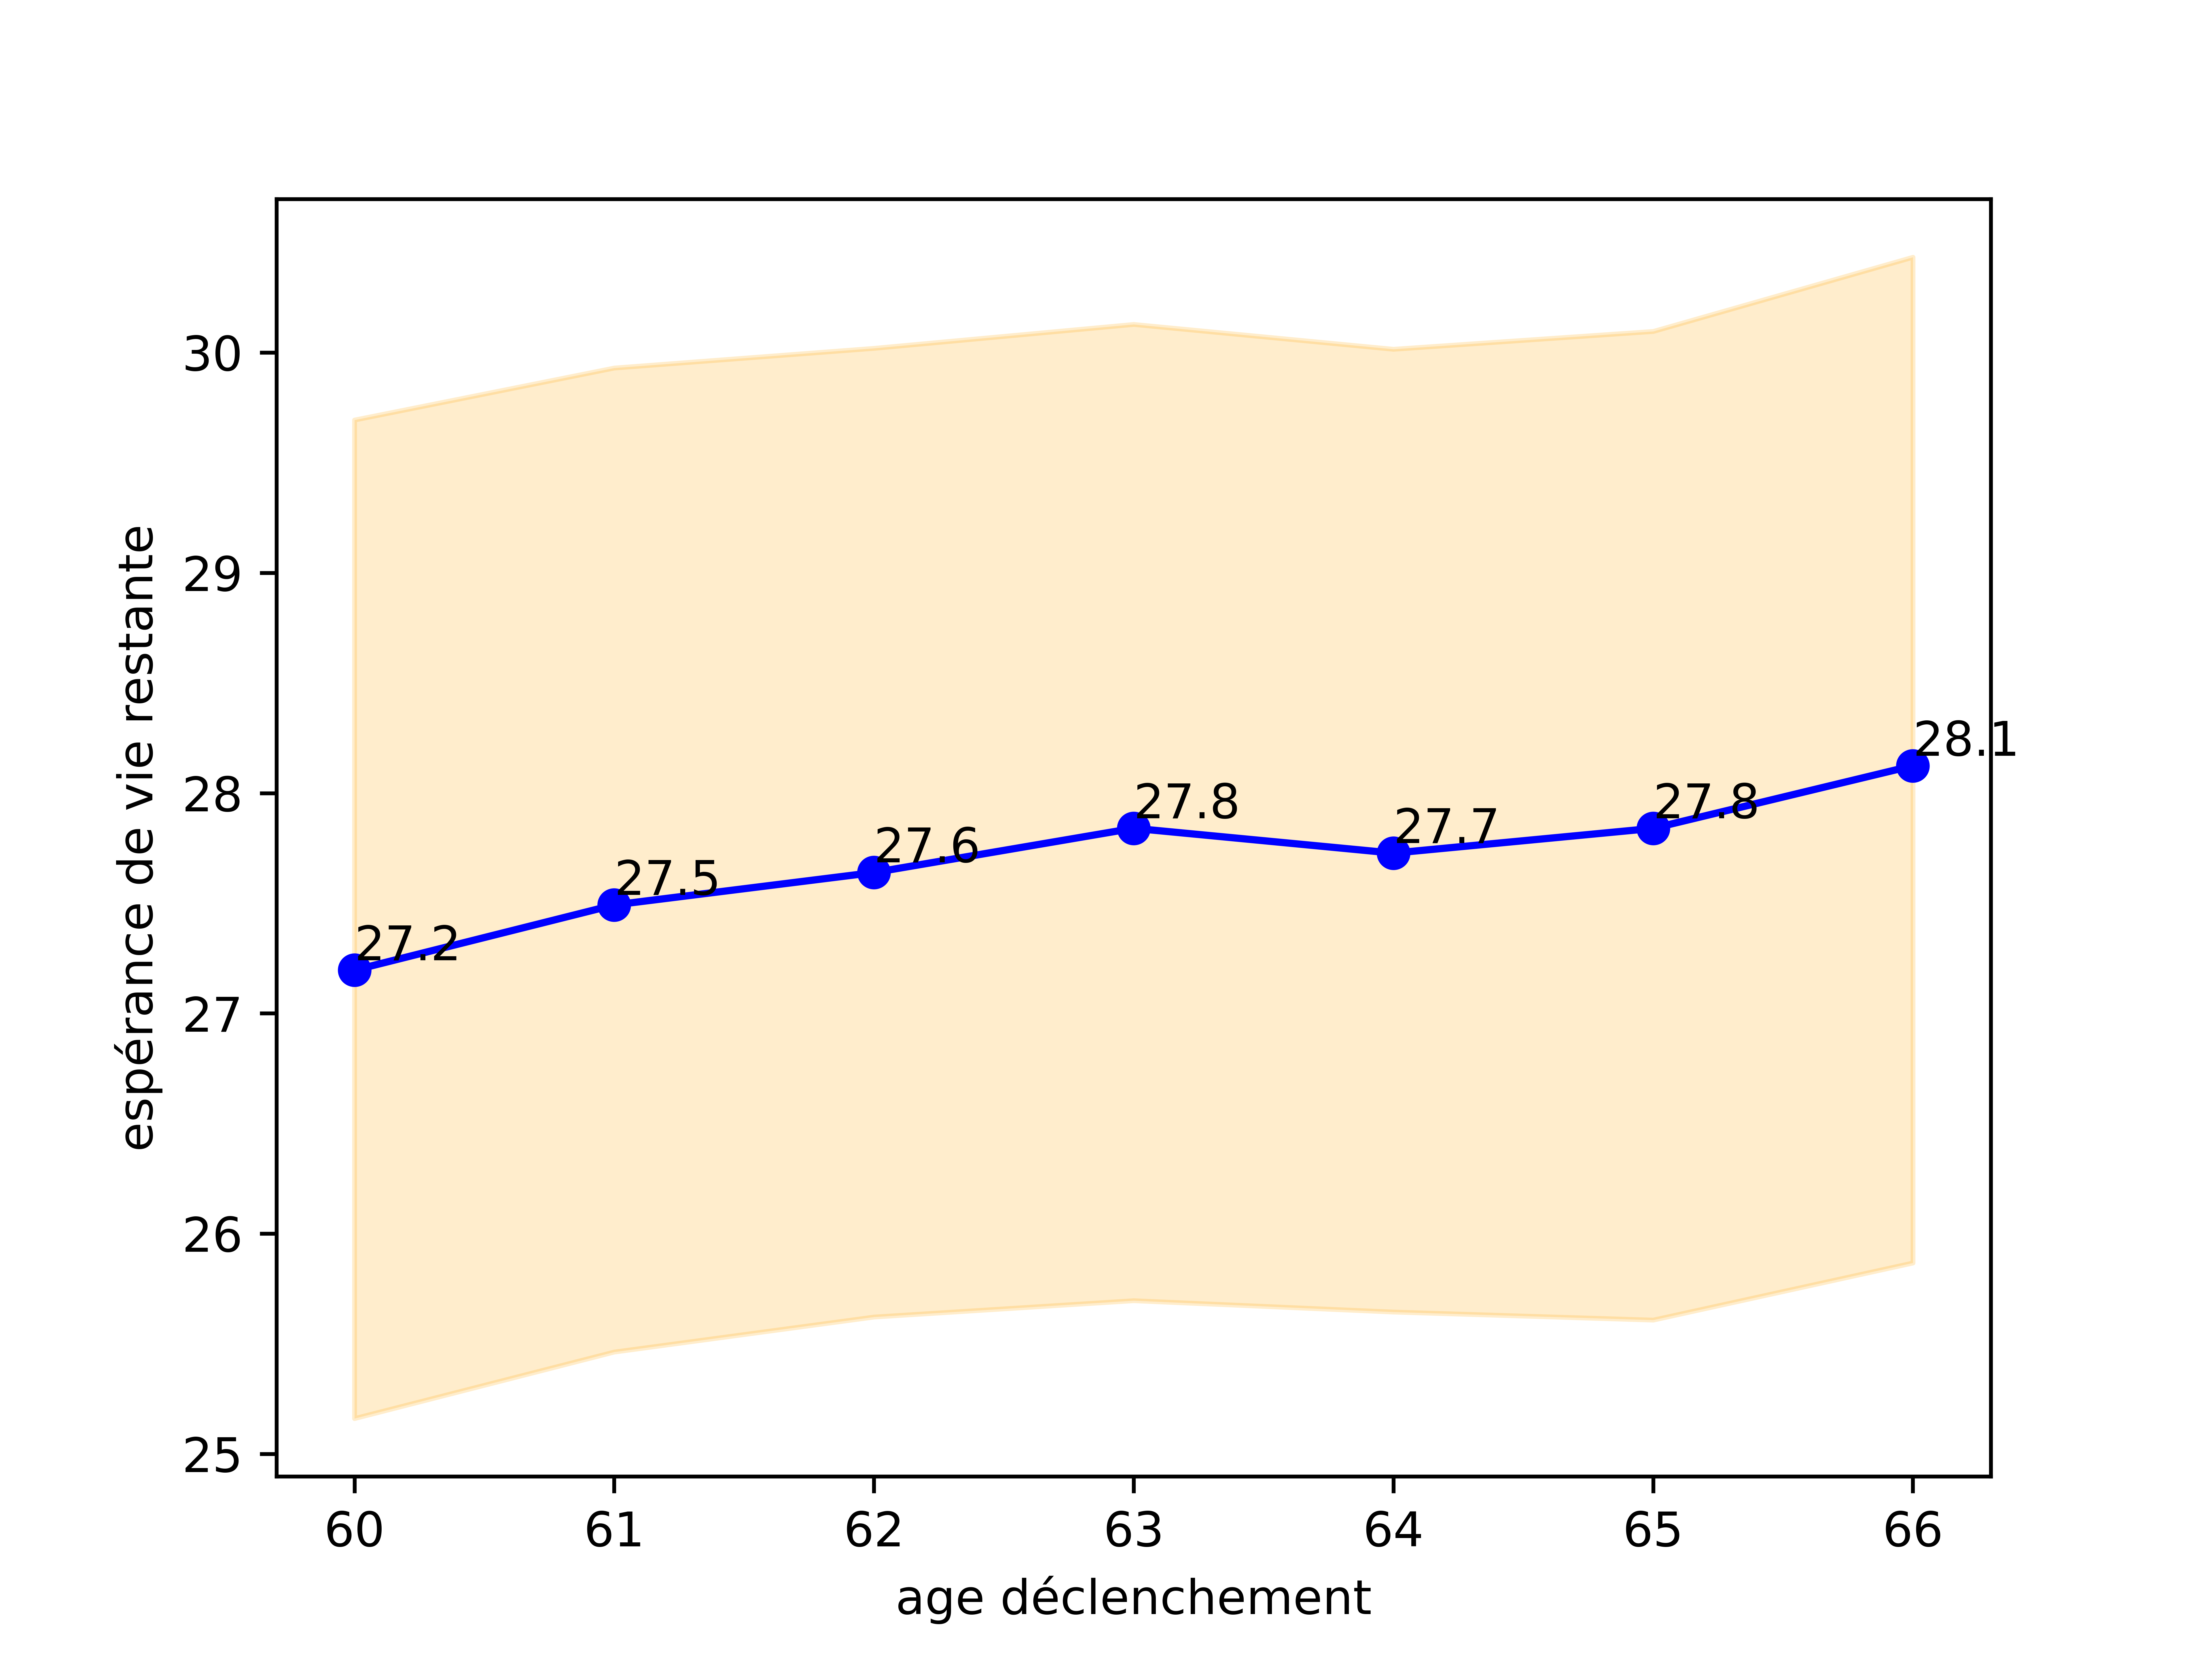
\includegraphics[scale=0.75]{../figures/ages.png}
	\caption{\textbf{Distribution des espérances de vie restante par âge de déclenchement de la RRQ} La médianne est présentée en bleu alors que la zone ombragée indique le 25e et le 75e percentile de la distribution.}
	\label{fig:ages}
\end{figure}
	
		
Une telle différence d'espérance de vie est-elle suffisante pour rationaliser de déclencher la rente à 60 ans? Pour répondre à cette questions,  attardons-nous à la valeur de retarder la rente pour ceux l'ayant débuté à 60 ans. La valeur d'un dollar de rente de retraite à 60 ans, étant donné que la rente est déclenchée à l'âge $c$, est de 
	
	$$ V_i(c) = a(c)\int_{c-60} s_{i}(t)e^{-rt}dt$$
	
où $a(c) = 1+\tau(c-65)$ est un facteur d'ajustement actuariel prescrit par le régime qui permet de bonifier la rente si le cotisant retarde le déclenchement (jusqu'à 65 ans).\footnote{Le facteur est plus élevé après 65 ans qu'avant 65 ans}. Dans le régime actuel, $\tau = 0.072$ pour ceux ayant droit à la rente maximale avant 65 ans.\footnote{Le régime du RRQ prévoit depuis 2014 une bonification qui dépend du niveau de la rente et donc implicitement des gains accumulés durant la vie afin de capturer la mortalité plus forte chez les moins fortunés.}  Le taux $r$ est une taux d'actualisation qui devrait capturer le rendement que peut obtenir le cotisant pour un profil de risque similaire. On utilise souvent le rendement obligataire pour ces comparaisons. Puisque la rente est indexée à l'inflation, il faut utiliser un taux réel. 
	 
Ainsi, pour deux âges, soit $60$ et $c$, $c>60$, Les valeurs présentes sont égales, $V_i(60) = V_i(c)$, si 
	
	
	$$a(60)\int_0 s_{i}(t)e^{-rt}dt = a(c)\int_{c-60} s_{i}(t)e^{-rt}dt .$$
	
	
	On peut donc définir le taux de rendement effectif du report de la rente en trouvant $r_i$ tel que 
	
	$$ q(r_i) =a(60) \int_0 s_{i}(t)e^{-r_i t}dt - a(c)\int_{c-60} s_{i}(t)e^{-r_i t}dt = 0$$
	
	Quelle interprétation donner à $r_i$? Puisque la rente de la RRQ est indexé à l'inflation, il s'agit du taux de rendement réel, sans risque (puisque le risque de défaut du régime est négligeable), nécessaire pour justifier de prendre sa rente à 60 ans plutôt qu'à l'âge $c$ et de l'investir. Si le taux qu'on pense obtenir en investissement sans risque et avec protection contre l'inflation est supérieur à $r_i$, l'investisseur gagne à prendre sa rente à 60 ans. 
	
	
	Étant donné la distribution de $\alpha_i$, $F(\alpha_i)$, nous pouvons obtenir la distribution de $r_i$ pour n'importe quel âge de déclenchement $c$. Le graphique suivant donne le taux de rendement effectif requis pour débuter sa rente à 60 ans plutôt qu'à 65 ans pour chaque niveau d'espérance de vie. La Figure \ref{fig:tri} présente les résultats. Même à un niveau d'espérance de vie faible, il faut espérer un rendement réel sans risque de plus de 3\% pour battre le report de la rente. Pour ceux ayant une espérance de vie moyenne, il faut espérer un rendement réel sans risque de plus de 6.5\%. Au printemps 2024, une obligation du gouvernement du Canada à long-terme avait un rendement nominal de 3.5\% alors que les obligations à rendement réel avaient un rendement de 1.6\%. Il est donc très peu probable de battre ce rendement à niveau de risque équivalent. 
	
	\begin{figure}[!htbp]
	\centering 
	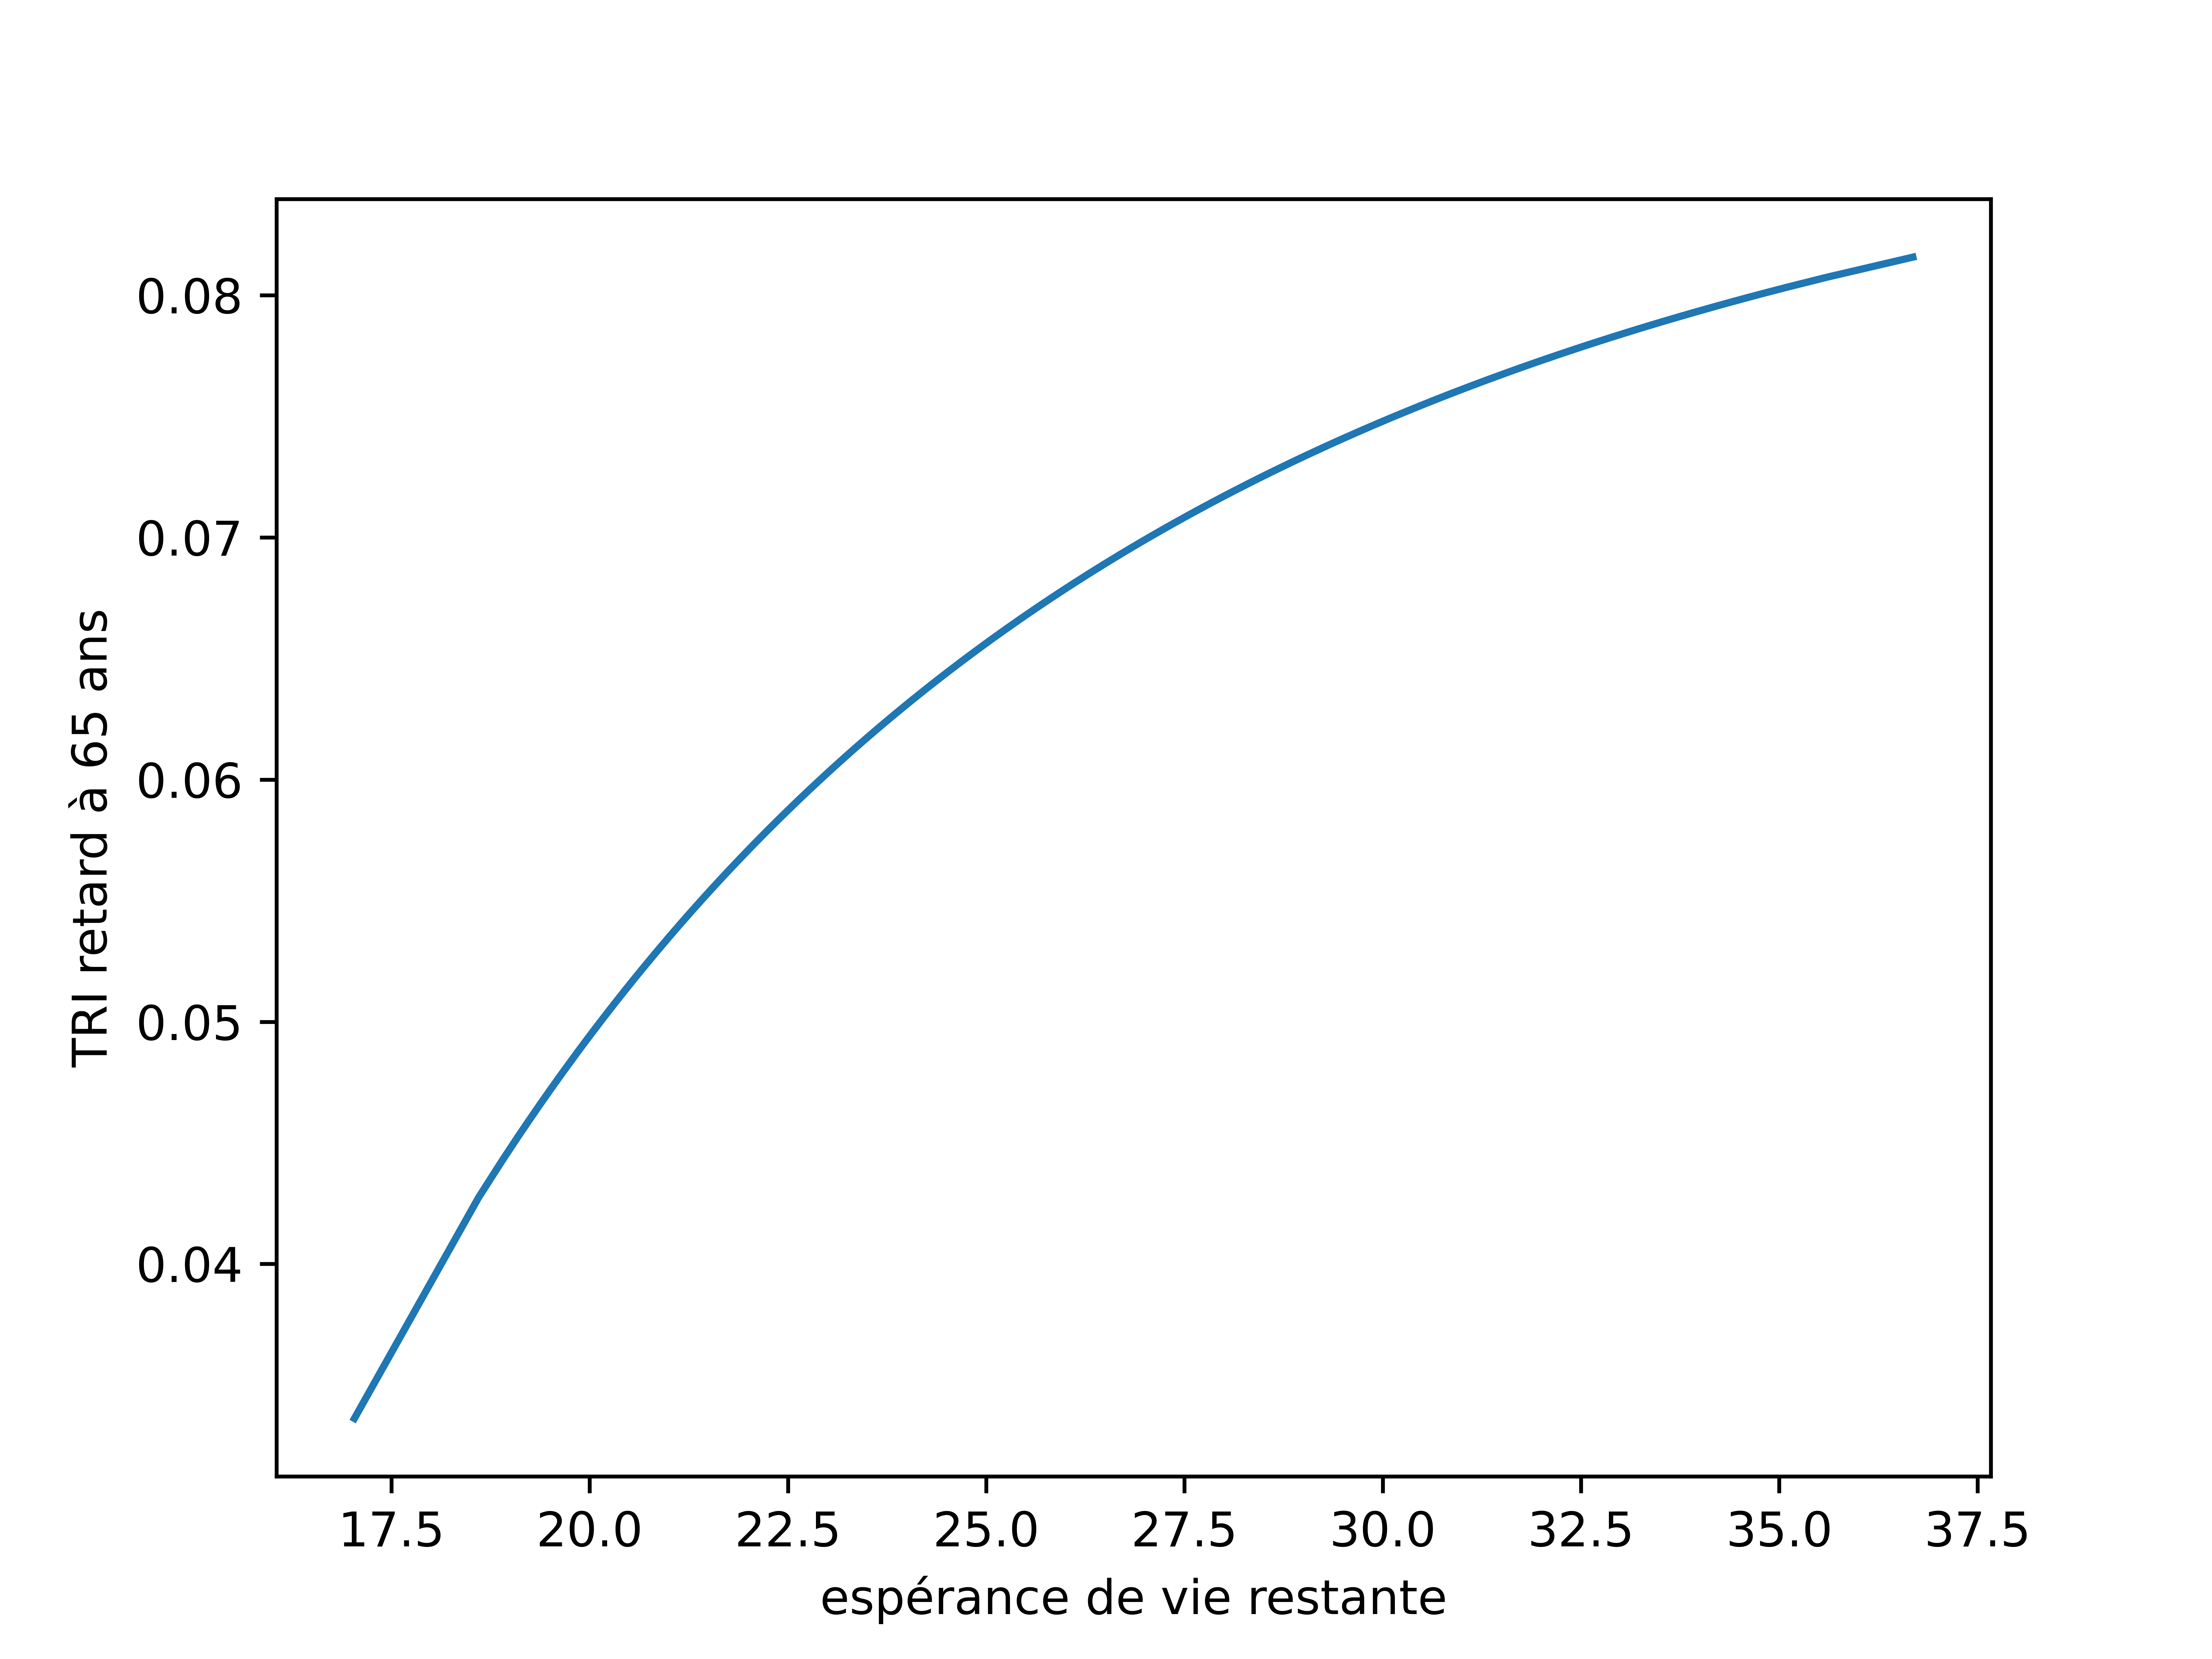
\includegraphics[scale=0.75]{../figures/tri.png}
	\caption{\textbf{Taux de rendement interne du report de la rente par niveau d'espérance de vie restante à 60 ans}}
	\label{fig:tri}
	\end{figure}	
	
	 
 	\newpage

	\section{Remplacement et déclenchement de la rente du RRQ}
	
	La suffisance du revenu à la retraite est une question compliquée. Quel est le bon niveau? Qu'est-ce qui est suffisant? Dans cette section, je veux m'intéresser aux revenus de retraite des retraités actuels en comparaison de leurs revenus avant la retraite. Ces revenus proviennent de plusieurs sources. De plus, l'impôt et différentes mesures fiscales affectent les revenus de retraite d'une manière différente qu'avant la retraite. Ainsi, je veux regarder une mesure du taux de remplacement, c'est à dire le ratio des revenus après la retraite et de ceux avant la retraite en utilisant une mesure des revenus après impôts et transferts. Si $y_2$ est ce revenu, disons entre l'âge de 70 et 74 ans, je veux calculer $\phi = \frac{y_2}{y_1}$ où $y_1$ est le revenu avant la retraite, disons entre l'âge de 55 à 59 ans.  Je vais calculer des statistiques sur $\phi$ par âge de déclenchement de la rente du RRQ. Je vais calculer la moyenne, la fraction avec un $\phi$ inférieur à 60\%, un niveau souvent jugé comme étant plutôt faible. Je vais aussi rapporter la moyenne de $y_1$ et $y_2$. Ces statistiques sont rapportées au Tableau 2. 
	

	\begin{table}[!htbp]
		\centering
		\begin{tabular}{lrr}
			\toprule
			
											& Début RRQ 60 ans & Début RRQ 65 ans \\
			\midrule
			Revenu avant retraite $y_1$ & 34600 & 43400 \\
			\midrule 
			Entre 66-69 ans  & & \\
			\multicolumn{1}{r}{$\phi$ moyen} & 112\% & 109\% \\
			\multicolumn{1}{r}{Fraction $\phi$<60\%} & 14.1\% & 16.3\% \\
			\multicolumn{1}{r}{Part revenu rentes} & 76.1\% & 46.1\% \\
			\midrule
			Entre 70-74 ans  & & \\
			\multicolumn{1}{r}{$\phi$ moyen} & 117\% & 103\% \\
			\multicolumn{1}{r}{Fraction $\phi$<60\%} & 15.2\% & 22.7\% \\	
			\multicolumn{1}{r}{Part revenu rentes} & 80.7\% & 60.9\% \\
			\bottomrule 
			
		\end{tabular}
		
		\caption{\textbf{Revenus et taux de remplacement selon l'âge de déclenchement}: Le tableau rapporte plusieurs statistiques de revenus selon l'âge de déclenchement. Le revenu après impôt moyen entre l'âge de 55-59 ans ($y_1$), le taux de remplacement moyen calculé de deux façons: individuel, soit $\phi = E_N \phi_i$, la moyenne des taux de remplacement calculée pour chaque cotisant. La part du revenu avant impôt qui est reçu sous forme de rentes (PSV, SRG, RRQ et revenus provenant d'un régime de retraite complémentaire). Ces statistiques sont produites pour deux groupes d'âge, soit entre 66-69 ans et ensuite entre 70 et 74 ans. }
	\end{table}
	
	On observe d'abord que les revenus avant la retraite sont plus élevés pour ceux retardant la rente que ceux la débutant à 60 ans. Ceux retardant ont donc des revenus plus élevés, avant même la retraite. Après la retraite, leurs revenus demeurent plus élevés. Quand on regarde la moyenne des taux de remplacement, ceux-ci sont très élevés, bien au delà de 100\%. Ceci est cohérent avec les résultats du CPR produit par l'Institut sur la Retraite et l'Épargne qui montrent que le taux de remplacement projeté moyen après impôts est près de 100\% \citep{ire2020}. Ceci est aussi cohérent avec les résultats de Statistique Canada montrant des taux de remplacement très élevés \citep{ostrovsky2010}. La fraction de cotisants ayant un taux de remplacement inférieur à 60\%, un niveau relativement faible, est généralement inférieur à 20\%. Cette fraction est plus élevée chez ceux retardant le déclenchement de la rente que chez ceux débutant la rente à 60 ans. On pourrait croire que ceux retardant jusqu'à 65 ans auront une part plus importante de leur revenu totaux provenant de rentes protégeant contre le risque de longévité. Or, ce n'est pas le cas. Entre 70 et 74 ans, ceux déclenchant à 60 ans ont une part de leur revenu provenant de rentes (des revenus relativement fixes) de plus de 81\% alors que cette part est de 61\% pour ceux retardant la rente. Ainsi, ceux déclenchant la rente tôt on en moyenne des revenus plutôt stable, avant même de considérer le report. 
	
	
	
	Puisque la distribution des taux de remplacement semble asymétrique, il pourrait être opportun de regarder comment varie les taux de remplacement par décile de la distribution des revenus après impôt avant la retraite (entre l'âge de 55 et 59 ans). La Figure \ref{fig:reprates} montre la moyenne de ces taux de remplacement par décile de revenu. Il est remarquable de voir comment les revenus à la retraite après impôts moyens sont en fait plus élevés qu'avant la retraite jusqu'au 5e décile. Même dans les déciles supérieurs, le taux de remplacement moyen est de plus 75\%. Ces taux de remplacement ne varient pratiquement pas selon l'âge de déclenchement de la rente du RRQ.  
	
	
	\begin{figure}[!htbp]
	\centering 
	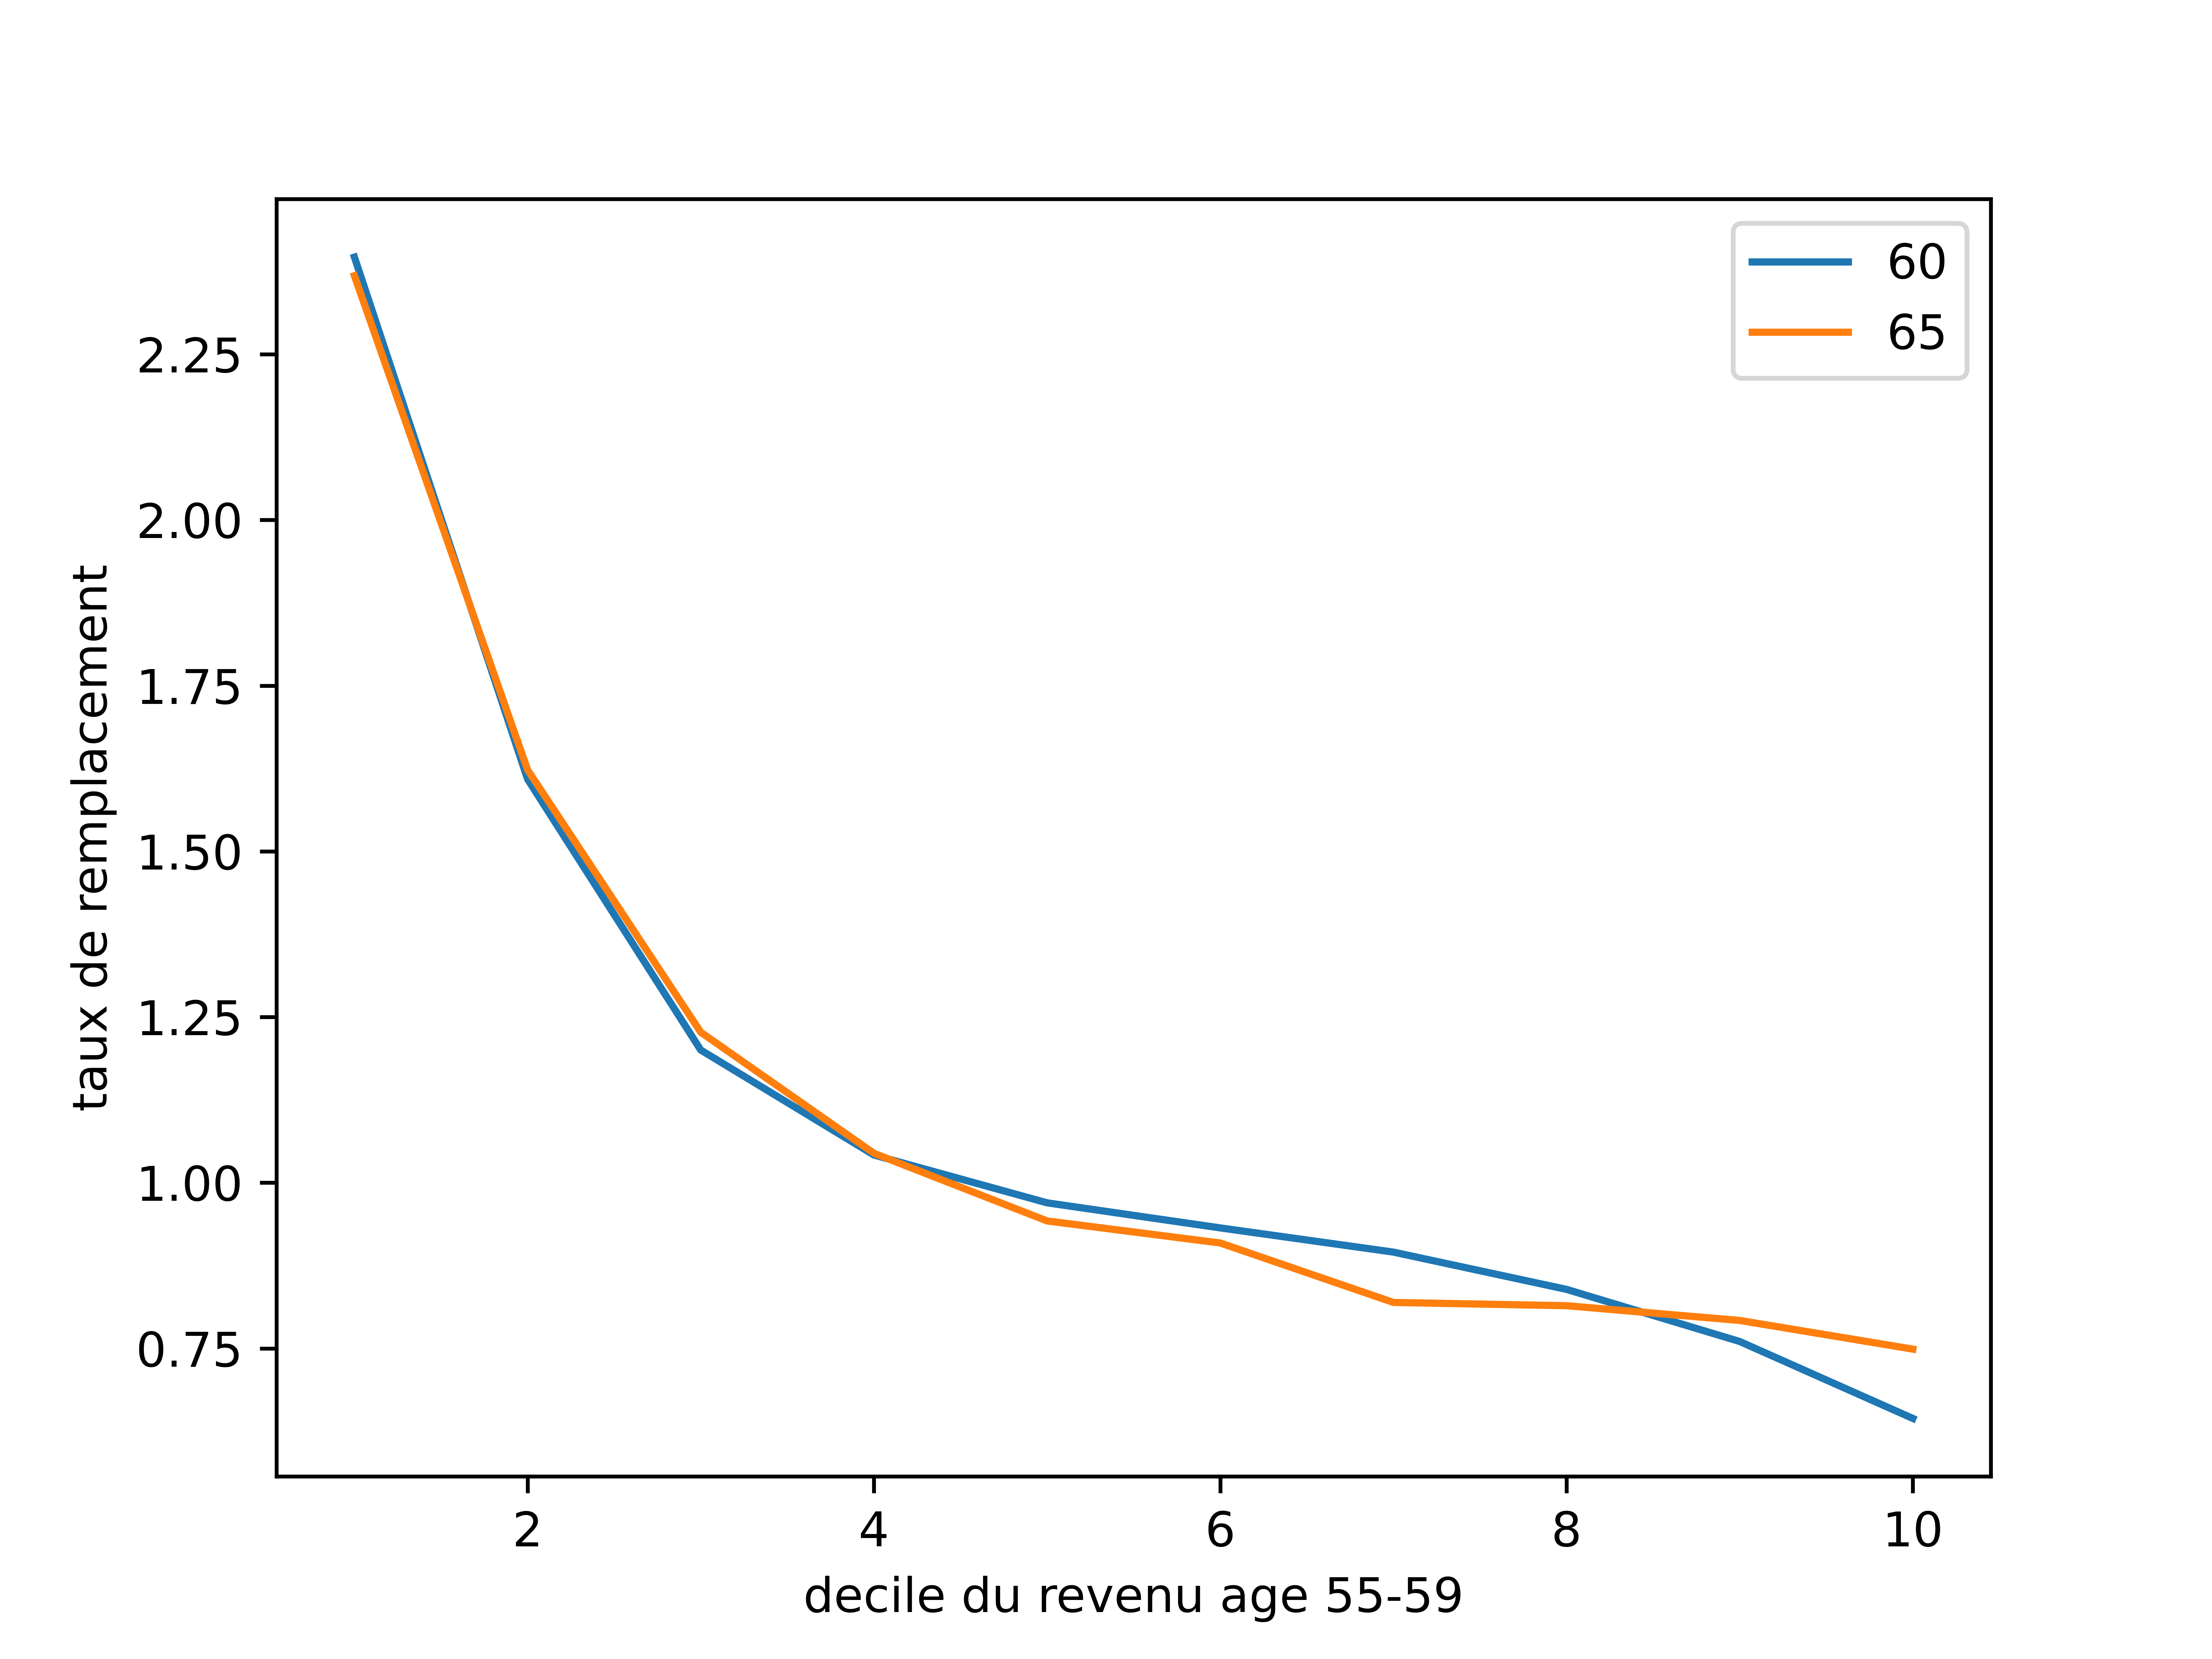
\includegraphics[scale=0.75]{../figures/reprates_decile.png}
	\caption{\textbf{Taux de remplacement après impôt selon le décile de revenu à l'age 55-59 ans}: La figure rapporte le taux de remplacement moyen $\phi = y_2/y_1$ selon le décile de la distribution de $y_1$, le revenu après impôt entre l'âge de 55 à 59 ans. Ces taux sont rapportés par âge de déclenchement (60 ou 65 ans). }
	\label{fig:reprates}
	\end{figure}		
	
	
	\section{Supplément de revenu garanti et rente du RRQ}
	
	Le report de la rente peut être financièrement bénéfique. Mais les revenus de retraite, notamment ceux provenant du supplément de revenu garanti, peuvent diminuer à partir de 65 ans si ceux du RRQ augmentent. En effet, le SRG est réduit en fonction du revenu imposable et les revenus de RRQ le sont. Le taux de récupération varie entre 50\% et 75\%. On pourrait penser que les revenus de RRQ ne seront pas touchés parce que ceux-ci s'ajoute à ceux de la pension de la vieillesse. Or les revenus de la PSV ne sont pas imposables. Ainsi, les premiers dollars touchés de RRQ seront généralement sujet à la récupération du SRG. Dans les données, nous pouvons calculer la fraction de cotisants qui reçoivent des revenus du SRG après 65 ans. Nous pouvons aussi calculer le revenu moyen de SRG qui est reçu. Nous faisons ce calcul pour chaque décile de revenu avant la retraite (55-59) et pour deux âge de déclenchement, soit 60 et 65 ans. 
	
	\begin{figure}[!htbp]
	\centering 
	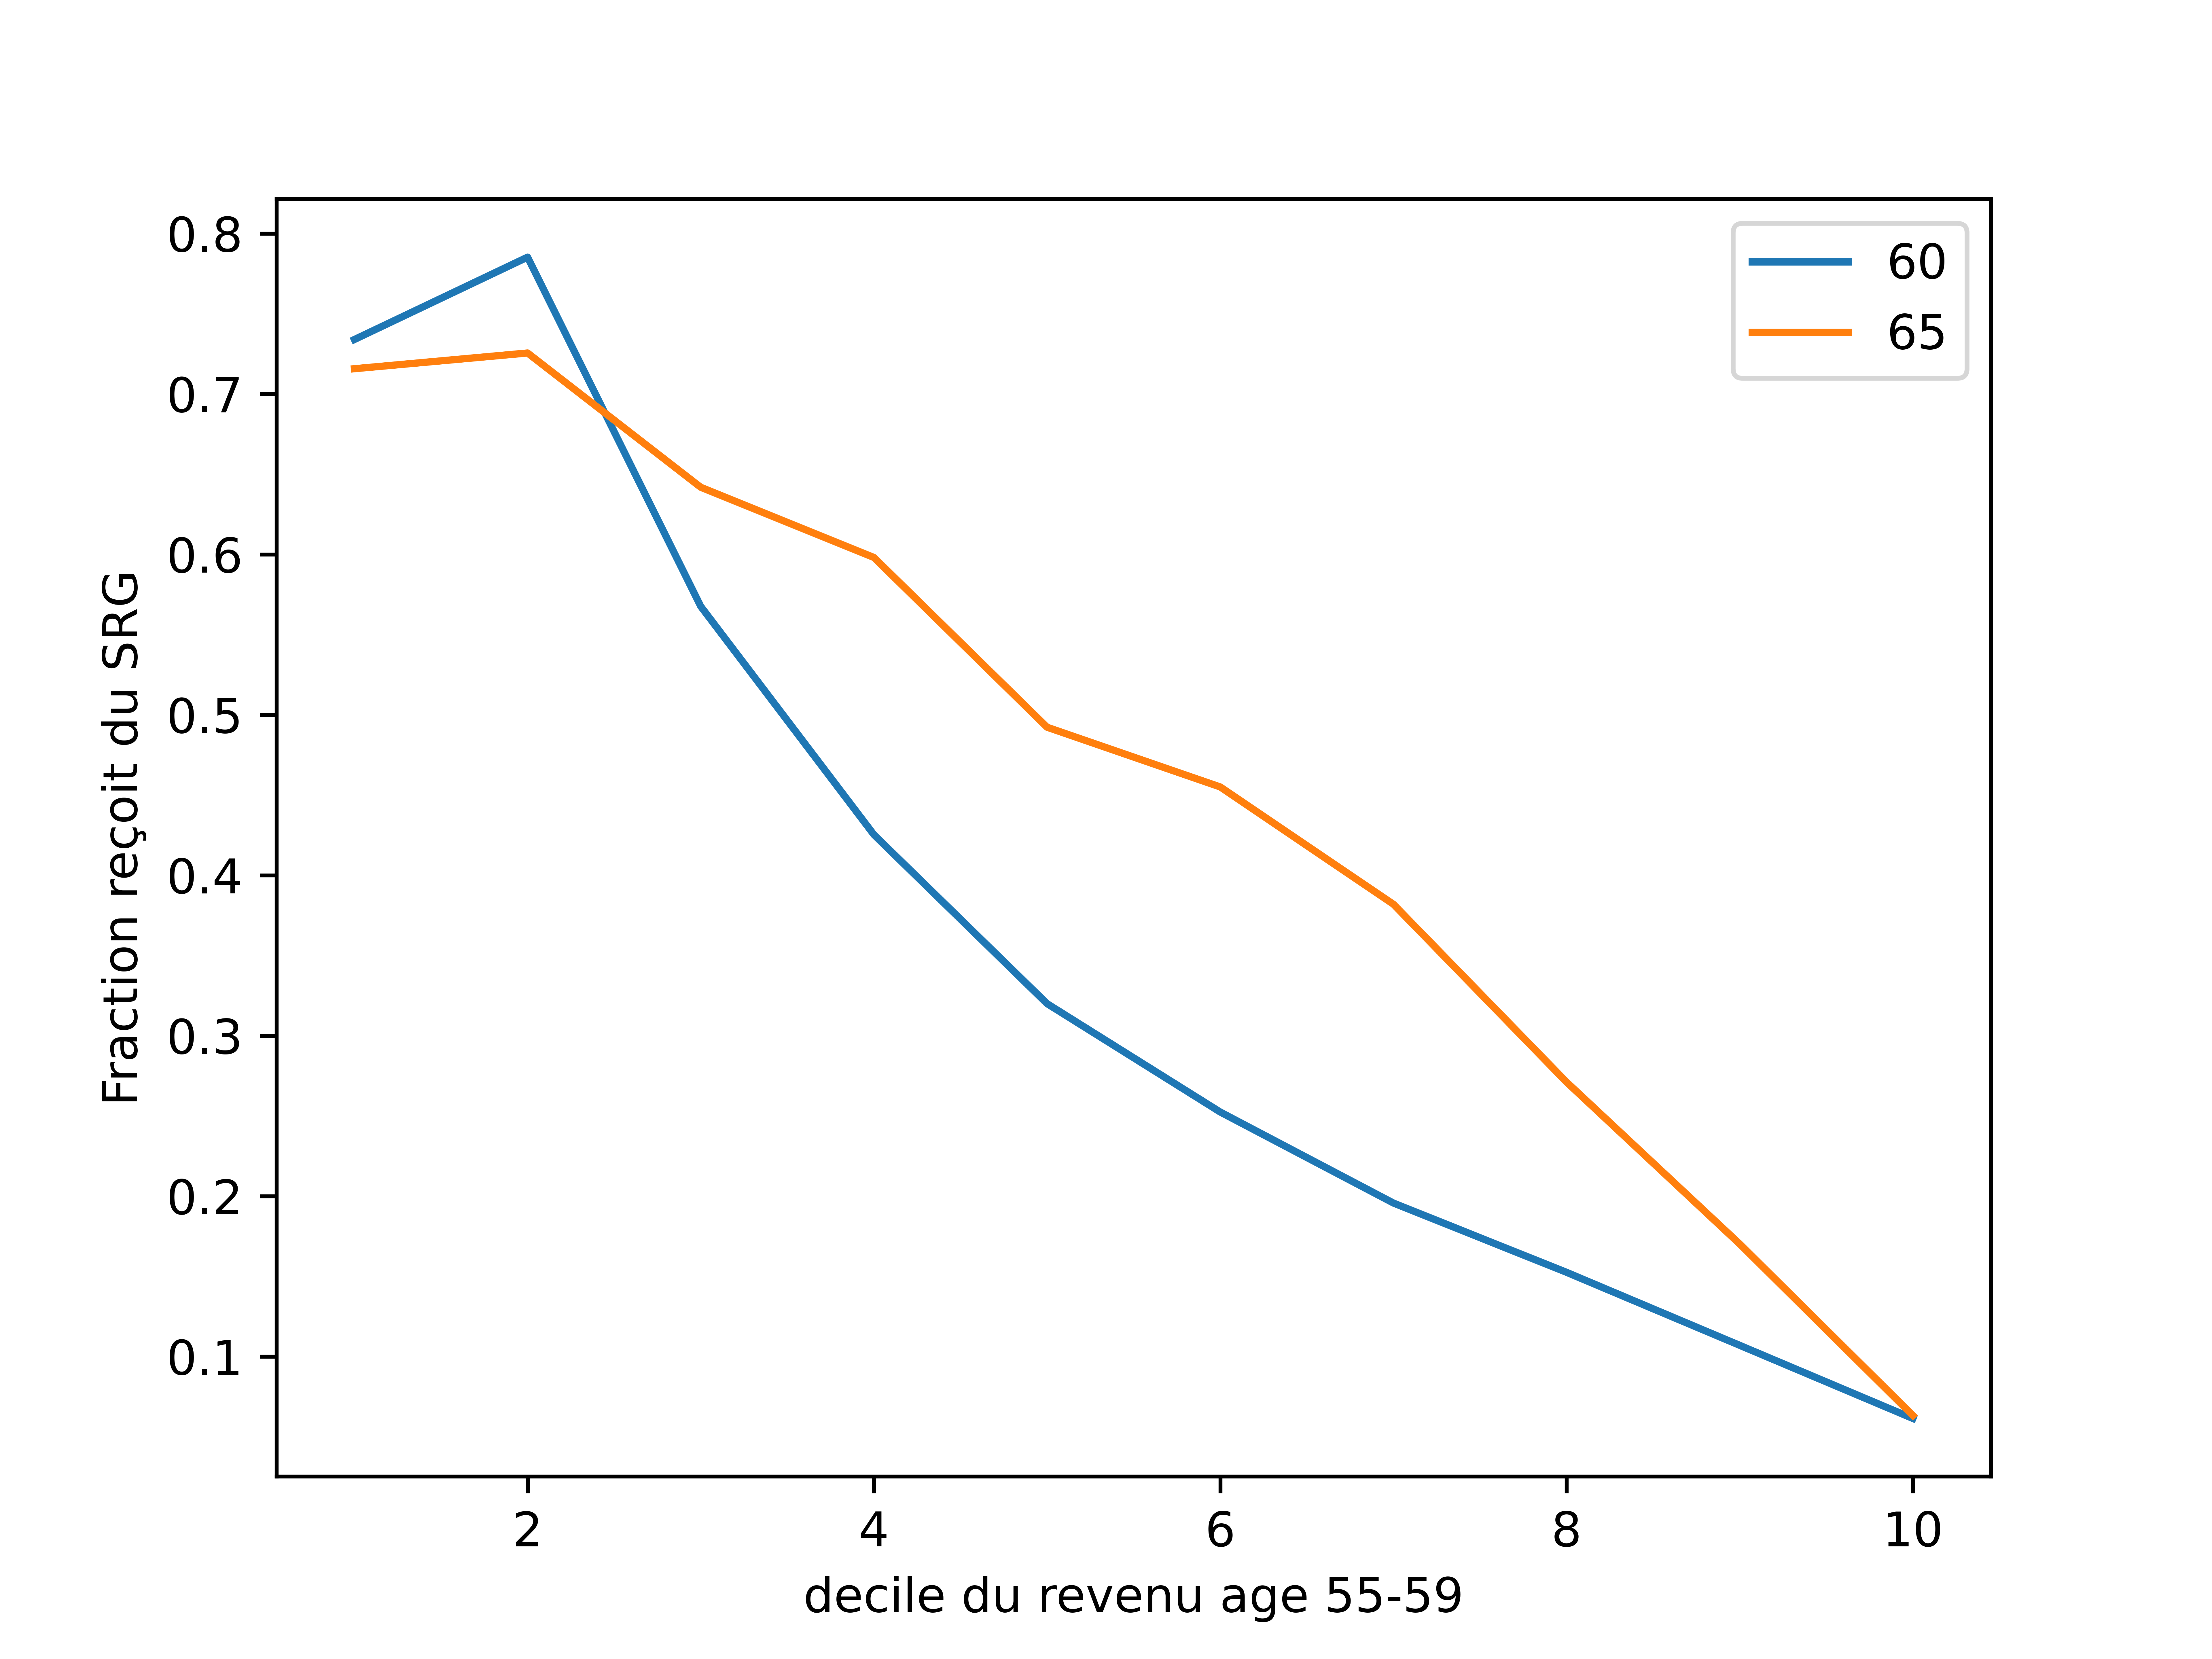
\includegraphics[scale=0.75]{../figures/srg_decile.png}
	\caption{\textbf{Proportion reçoit des revenus de SRG entre 70-74 ans selon le décile de revenu à l'age 55-59 ans}}
	\label{fig:gis}
	\end{figure}		
	
	Puisque le SRG est un programme de soutien du revenu pour ceux ayant des revenus faibles, il n'est pas surprenant qu'une grande majorité (entre 70 et 80\%) des cotisants dans les premiers décides de revenus avant la retraite reçoivent des revenus provenant du SRG. Cette proportion diminue avec le revenu mais elle demeure élevée même parmi ceux ayant des revenus à la médiane. Cette proportion varie selon l'âge de déclenchement. Elle est plus élevée chez ceux retardant la rente que chez ceux débutant la rente à 60 ans. Ainsi, cette question de la récupération du SRG, et comment ceci affecte le rendement de reporter la rente s'applique à beaucoup de cotisants. 
	
	Afin de voir plus clair, nous allons calculer le gain net moyen, pour chaque dollar de bonification de rente à partir de 65 ans. Nous prenons tous les cotisants ayant débuter leur rentre à 60 ans et regardons ce qu'il resterait net dans leur poche à partir de 65 ans pour chaque dollar additionel de RRQ reçu à partir de 65 ans. La Figure \ref{fig:claw} montre les résultats de ce calcul par décile du revenu avant 60 ans. On observe qu'au bas de la distribution, il restrait en moyenne moins de 65 cent par dollar additionnel de rente. Il y a donc une taxe implicite moyenne de 35 pourcent sur le report de la rente. Cette taxe diminue avec le revenu mais dev ient inférieur à 10\% seulement à partir la médiane. Donc, plus de la moitié des cotisants ayant débuté leur rente à 60 ans aurait eu une taxe de plus de 10\% sur le report de la rente.   
	
	
	\begin{figure}[!htbp]
	\centering 
	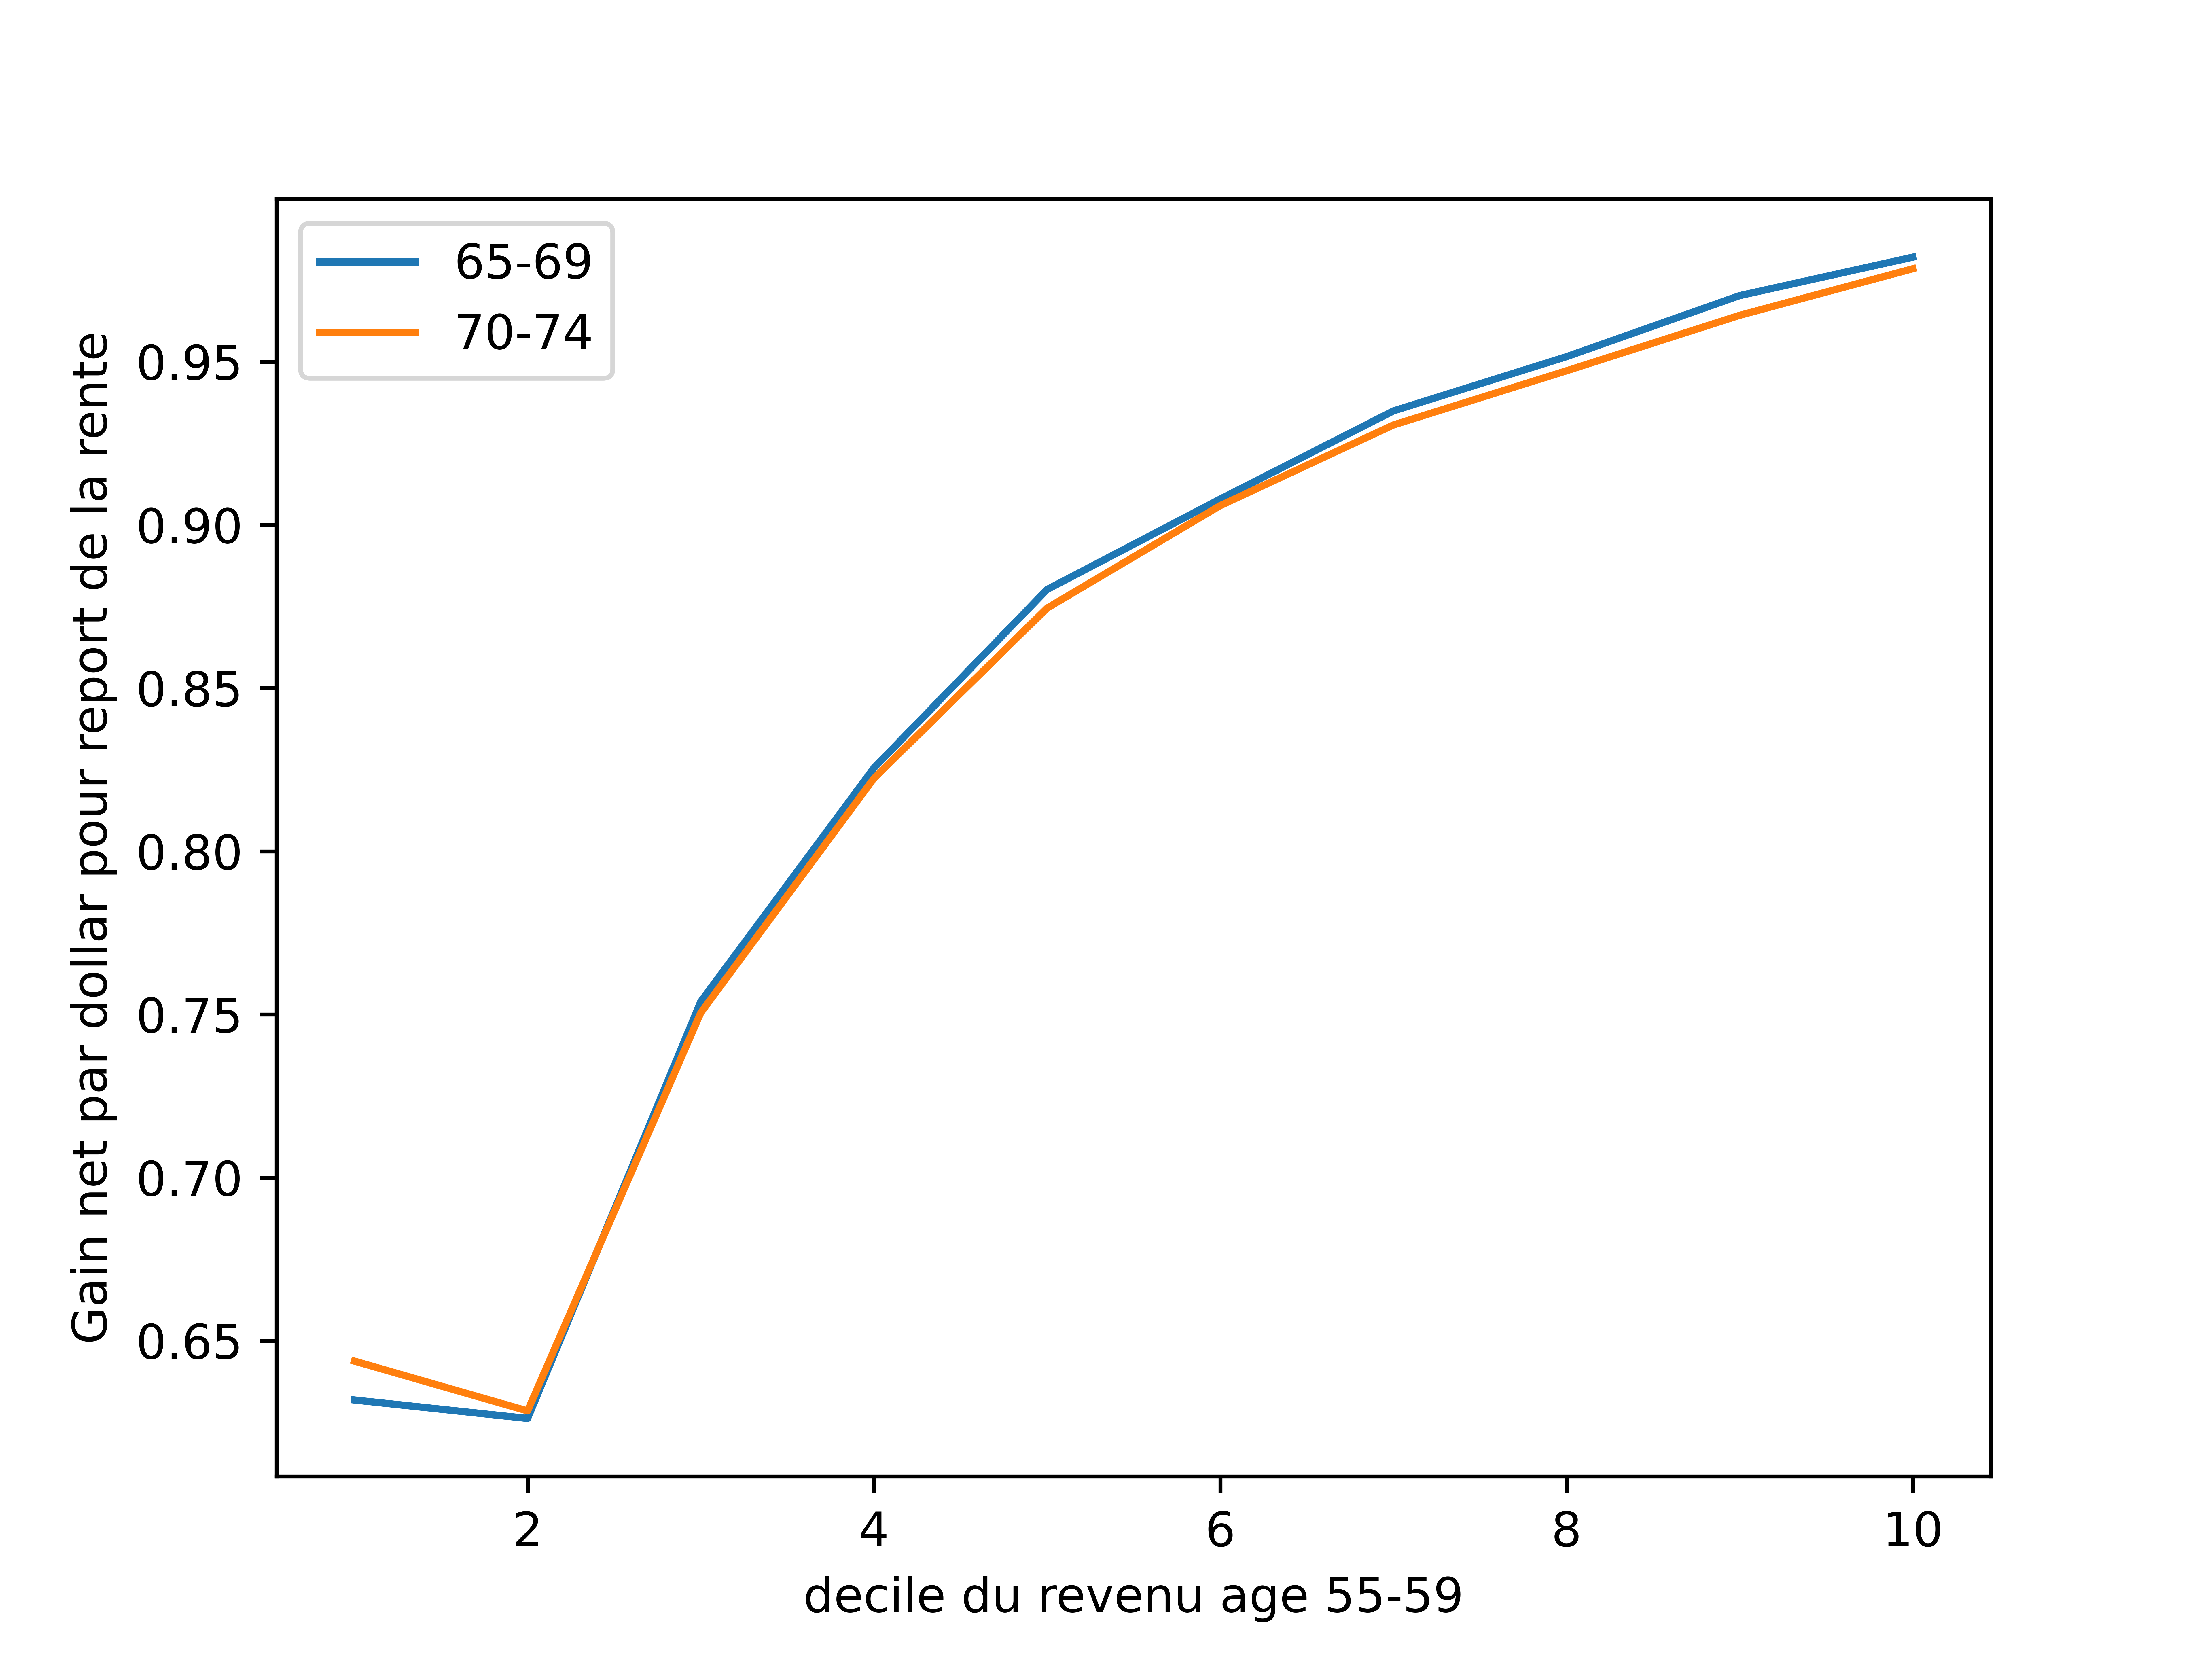
\includegraphics[scale=0.75]{../figures/claw_decile.png}
	\caption{\textbf{Gain net de reporter la rente par dollar selon le décile de revenu à l'age 55-59 ans}}
	\label{fig:claw}
	\end{figure}
	
	Pour bien illustrer comment ceci affecte le rendement effectif du report, on peut revenir à la définition du rendement effectif. La valeur d'un dollar de rente si celle-ci début à l'âge $c$ est maintenant 
	
	$$ V_i(c) = a(c)\int_{c-60} s_{i}(t)e^{-rt}dt$$
		
	Nous pouvons reprendre notre calcul du taux de rendement effectif. Nous avons maintenant 
	
	$$ q(r_i) = a(60)\int_0 s_{i}(t)e^{-r_i t}dt - a(c)\int_{c-60} s_{i}(t)e^{-\theta_iI(t>65)}e^{-r_i t}dt = 0$$
	
	où $\theta_i$ est la perte de revenu net moyenne provenant de la récupération. Tel que démontré à la Figure \ref{fig:claw}, cette pénalité est en moyenne entre 5 et 35\%. À la Figure \ref{fig:tri_claw}, nous avons calculé le taux de rendement effectif par décile de revenu avant la retraite en prenant la mortalité moyenne par niveau de revenu. Sans surprise, le rendement effectif est beaucoup plus faible pour les déciles inférieurs. Ces dans les deux premiers déciles ont un rendement réel effectif de moins de 3\%. La domination du report est beaucoup moins évidente et dépendra du rendement sur les placements alternatifs ajusté pour le risque. Le rendement demeure néanmoins plus élevé qeu celui d'une obligation réelle de long-terme. 
	
	\begin{figure}[!htbp]
	\centering 
	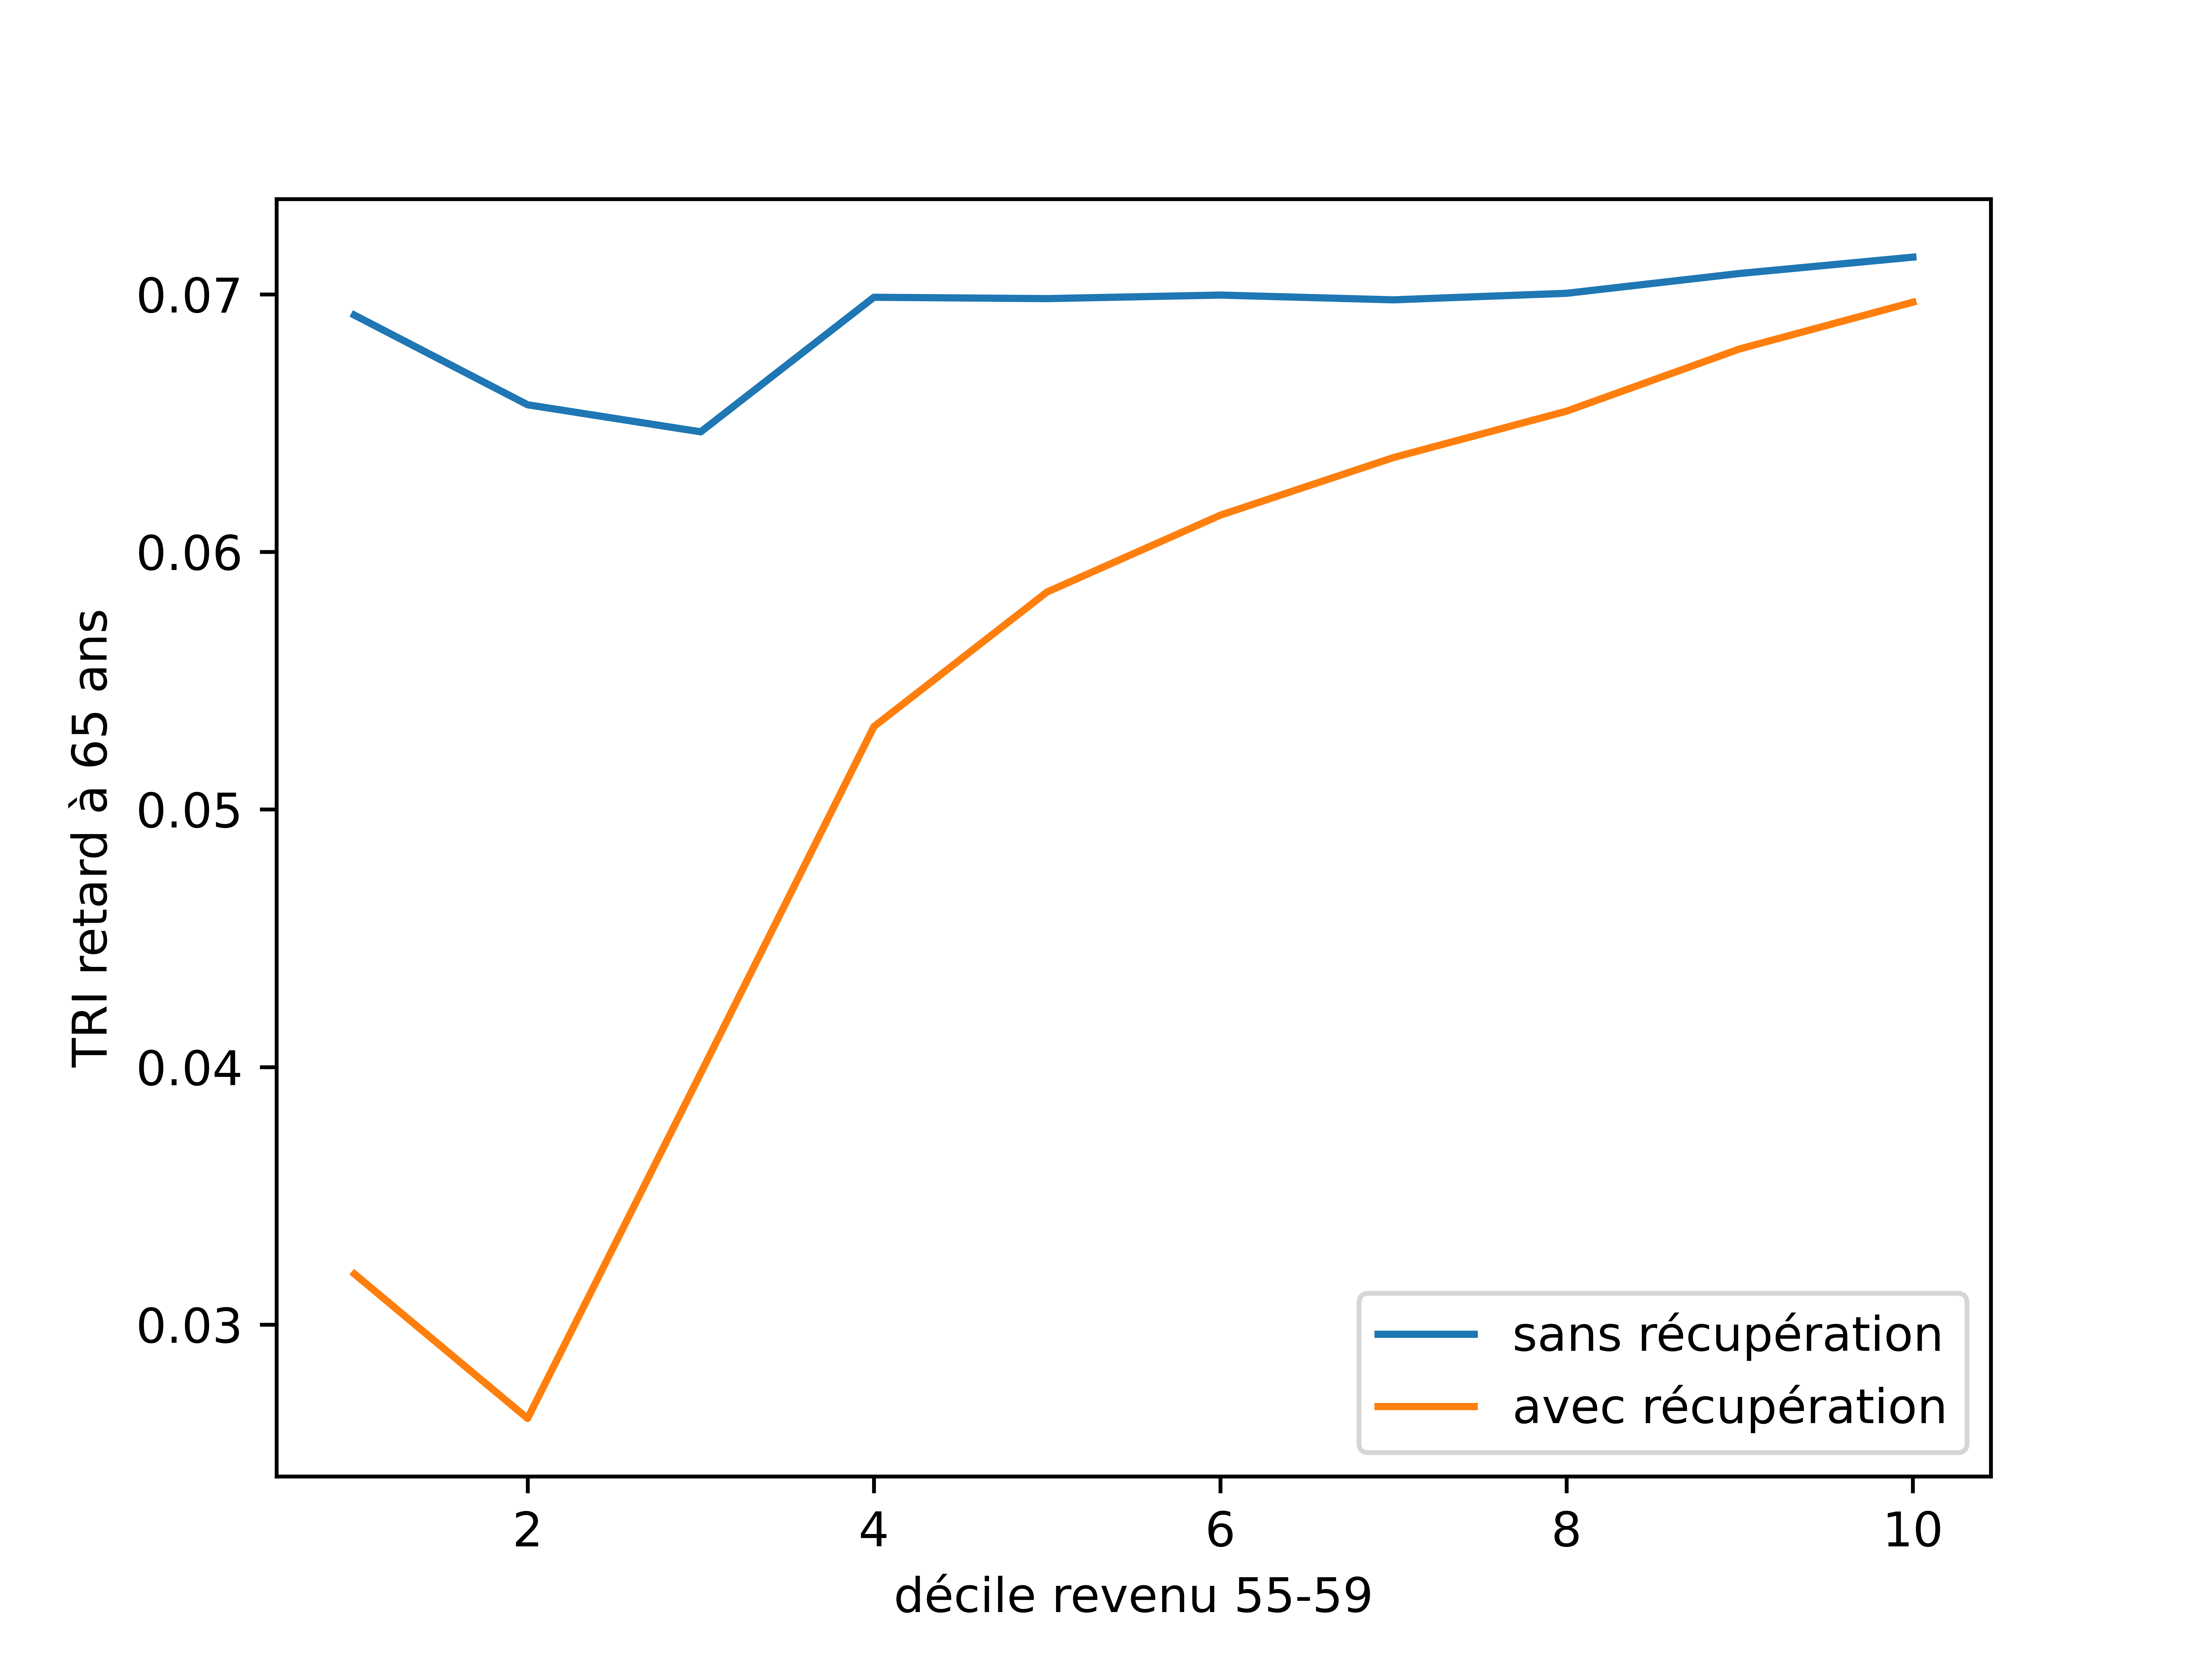
\includegraphics[scale=0.75]{../figures/tri_claw.png}
	\caption{\textbf{Taux de rendement interne du report de la rente par niveau d'espérance de vie restante à 60 ans selon la récupération effective moyenne du SRG}}
	\label{fig:tri_claw}
	\end{figure}
	
	Le taux de rendement d'une obligation réelle n'est cependant pas probablement le bon taux de comparaison. Ceci dépendra de la source des fonds qui fiancerait la consommation pendant les années où le report est effectué. Par exemple, si le cotisant utilise des fonds d'épargne qui sont investis dans un RÉER, il faut comprendre que la sortie de ces fonds après l'âge de 65 ans aurait aussi mené à une récupération en terme du SRG. Ainsi, il ne faut pas prendre en compte la récupération du SRG dans le calcul puisque les deux stratégies (report ou non) entraîne une récupération. Si les fonds proviennent plutôt d'un CELI, on peut utiliser ce taux sur une obligation réelle. Finalement, si les fonds proviennent d'un compte d'épargne imposable, alors il faut utiliser le taux de rendement après impôt. 
	
	
	\section{Conclusion}
	
	Dans cet article, notre objectif était de revenir sur la question du report de l'âge de déclenchement de la rente RRQ. Nous voulions en particulier mettre en valeur des données fiscales inédites qui n'avaient pas été encore utilisée pour bien représenter l'hétérogénéité de la longévité au Québec. Par ailleurs, nous voulions aussi faire un état des lieux des taux de remplacement après impôt réalisé chez les cotisants québécois. Ceci permet de juger de la désirabilité du report de la rente afin d'augmenter le taux de remplacement à la retraite. Finallement, nous voulions regarder si la pénalité venant de la récupération du SRG étant bien réelle pour les retraités québécois. 
	
	Nos résultats montrent d'abord que la longévité est distribuée de manière très inégale au Québec. Plus de 10\% des retraités au Québec ont une espérance de vie à 60 ans inférieure à 24 ans alors que plus de 10\% ont une espérance de vie supérieure à 31.5 années. Il s'agit d'une différente non-négligeable de 7 années. Malgré le fait que les cotisants déclenchant la rente à 60 ans ont en moyenne une espérance de vie plus faible que ceux retardant le déclenchement, les progrès de l'espérance de vie font en sorte qu'il est avantageux pour presque tous les profils de retarder la rente de retraite, au moins jusqu'à l'âge de 65 ans. C'est plutôt du côté de la récupération du SRG qu'il faut regarder pour un motif financier afin de déclencher la rente à 60 ans. Beaucoup de québécois recoivent du SRG après 65 ans, en particulier ceux ayant des revenus inférieurs à la médianne avant l'âge de 60 ans. Pour ces gens, la pénalité réduit en moyenne l'augmentation de la rente provenant du report de près de 35 cents pour chaque dollar supplémentaire de rente. Cette pénalité réduit substentiellement le rendement effectif du report de la rente. Il convient cependant de bien comprendre que le taux de rendement comparatif à utiliser dépendra de la source des fonds qui financement la consommation pendant les années où le report est effectué. 
	
	Un résultat intéressant de cet article, mais qui confirme d'autres calculs effectués par le passé, est que le taux de remplacement après impôt est en moyenne très élevé au Québec, dépassant en moyenne 100\%. Une minorité de cotisants, moins de 20\%, ont des taux de remplacement inférieur à 60\%. Ces taux de remplacement ne sont pas plus faible chez ceux débutant la rente à 60 ans. Ainsi, il n'est pas vrai que ces cotisants sont moins en mesure de maintenir leur niveau de vie à la retraite, du moins en terme de revenu après impôt. 
	
	À la lumière de ces résultats, certaines recommendations peuvent être faites. D'abord, l'éducation concernant la hausse de la longévité, la récupération par le SRG, semble être une mesure à priviliéger afin d'aider les cotisants à déterminer un âge de déclenchement qui leur est bénéfique, dû moins financièrement. État donné les progrès de l'espérance de vie, il pourrait devenir pertinent pour le régime d'augmenter la pénalité pour un début hatif de la rente du RRQ dans les années à venir. Ce que gagne les cotisants à retarder est une perte financière pour le régime, ce qui demande de maintenir un taux de contribution artificiellement plus élevé qu'il ne devrait l'être. Il sera aussi important de bien expliquer aux cotisants que le rendement alternatif au report doit être considérable, une fois ajusté pour le risque et l'inflation, pour justifier de prendre sa rente plus rapidement. 
	
	Il est important de souligner que la décision de l'âge optimal pour déclencher la rente est une question qui n'est pas strictement financière. Étant donné le taux de remplacement déjà élevé pour un grand nombre de ménage, la demande de rente viagère additionelle de ceux-ci est probablement faible dans un contexte de modèle de cycle de vie. Ceci est probablement vrai dans un contexte où les retraités auraient un motif d'héritage important. Dans ce contexte, ils ne voudront financier un report en utilisant l'épargne qu'il voudrait laisser en héritage. 
	
	Par ailleurs, il est aussi important de souligner que l'état de santé futur, pour une espérance de vie donnée, l'espérance de vie en santé, peut aussi affecter ce calcul. Si l'utilité marginale de la consommation est plus faible en mauvaise santé, le besoin d'annuitisation sera encore plus faible aux âges avancées. Dans ce cas, l'optimalité du report risque d'être encore plus faible. D'un autre côté, l'aversion au risque est un élément important dans ce calcul d'optimalité. Si le placement alternatif au report de la rente est risqué, un individu averse au risque sera prêt à payer davantage pour une rente qui élimine ce risque. Dans un avenir rapproché, il pourrait être intéressant de faire ces calculs afin de bien dégager la valeur économique du report de la rente. Toutes ces considérations mettent en garde contre une recommandation mur à mur de retarder la rente pour tous les cotisants. La sensibilisation aux gains de report peut certes devenir un objectif adéquat en terme de politique publique, mais un jugement paternaliste menant à une solution de report obligatoire nous apparait inopportun étant donné l'état des connaissances sur les préférences des cotisants québécois.  
	 
	
	\newpage
	\clearpage
	\bibliography{refs}
	\newpage
	

	
	\newpage 
	
	
\end{document}
